% This document describes the ee know-how used in Qucs.

\documentclass[10pt]{report}
\usepackage{a4wide}
\usepackage{epsfig}
\usepackage{array}
\usepackage{amsmath}
\usepackage{SIunits}
\usepackage{psfrag}
\usepackage{relsize}
\usepackage[section]{placeins}
\usepackage{listings}

\newif\ifpdf
\ifx\pdfoutput\undefined
  \pdffalse
\else
  \pdfoutput=1
  \pdftrue
\fi

\ifpdf
\pdfcompresslevel=9
\pdfinfo {
  /Title   (Qucs)
  /Subject (Technical Papers)
  /Author  (Stefan Jahn)
}
\fi

\makeatletter
\def\thickhrulefill{\leavevmode \leaders \hrule height 1pt\hfill \kern \z@}
\renewcommand{\maketitle}{\begin{titlepage}%
    \let\footnotesize\small
    \let\footnoterule\relax
    \parindent \z@
    \reset@font
    \null\vfil
    \vspace*{3cm}
    \begin{flushleft}
      \bf \huge \@title
    \end{flushleft}
    \par
    \hrule height 3pt
    \par
    \begin{flushright}
      \LARGE Technical Papers \par
    \end{flushright}
    \vskip 60\p@
    \vfill


    \begin{flushright}
      \Large \@author \par
    \end{flushright}

    \hrule height 3pt \par

\vspace*{24pt}

Copyright \copyright{} 2003, 2004 Michael Margraf 
\textless michael.margraf@alumni.tu-berlin.de\textgreater \par
Copyright \copyright{} 2003, 2004 Stefan Jahn 
\textless jahn@mwt.ee.tu-berlin.de\textgreater \par

\vspace*{12pt}

Permission is granted to copy, distribute and/or modify this document
under the terms of the GNU Free Documentation License, Version 1.1 or
any later version published by the Free Software Foundation.  A copy
of the license is included in the section entitled "GNU Free
Documentation License".

\vspace*{1cm}

  \end{titlepage}%
  \setcounter{footnote}{0}%
}
\makeatother

\author{Michael Margraf \\ Stefan Jahn}
\title{Qucs}
\date{}

\begin{document}

\maketitle

\tableofcontents

\setlength{\parindent}{0pt}
\newpage

\chapter{Scattering parameters}
%\addcontentsline{toc}{chapter}{Scattering parameters}

\section{Introduction and definition}
%\addcontentsline{toc}{section}{Introduction and definition}

Voltage and current are hard to measure at high frequencies.  Short
and open circuits (used by definitions of most n-port parameters) are
hard to realize at high frequencies.  Therefore, microwave engineers
work with so-called scattering parameters (S parameters), that uses
waves and matched terminations (normally $50 \Omega$).  This procedure
also minimizes reflexion problems.

\addvspace{12pt}

A (normalized) wave is defined as ingoing wave $\underline{a}$ or
outgoing wave $\underline{b}$:

\begin{equation}
\underline{a} = \frac{u+Z_0\cdot i}{\sqrt{\text{Re}(Z_0)}} \qquad
\underline{b} = \frac{u-Z_0^*\cdot i}{\sqrt{\text{Re}(Z_0)}}
\label{equ:waves}
\end{equation}
where $u$ is (peak) voltage, $i$ (peak) current and $Z_0$ reference
impedance. The waves are related to power in the following way.
\begin{equation}
P = \frac{1}{2}\cdot \left( |\underline{a}|^2 - |\underline{b}|^2 \right)
\end{equation}
Now, characterizing an n-port is straight-forward:
\begin{equation}
\begin{pmatrix}
\underline{b}_1\\
\vdots\\
\underline{b}_n\\
\end{pmatrix}
=
\begin{pmatrix}
\underline{S}_{11} & \ldots & \underline{S}_{1n}\\
\vdots & \ddots & \vdots\\
\underline{S}_{n1} & \ldots & \underline{S}_{nn}\\
\end{pmatrix}
\cdot
\begin{pmatrix}
\underline{a}_1\\
\vdots\\
\underline{a}_n\\
\end{pmatrix}
\end{equation}


\section{Computing with S-parameters}
%\addcontentsline{toc}{section}{Computing with S-parameters}

\subsection{Recalculating $\mathbf{50\ohm}$-S-parameters for arbitrary port impedances}
%\addcontentsline{toc}{subsection}{Recalculating $50\ohm$-S-parameters for arbitrary port impedances}

During S-parameter usage it sometimes appears to have not all components
in a circuit normalized to the same impedance. But calculations can only
be performed with all ports being normalized to the same impedance. In
the field of high
frequency techniques this is usually $50\ohm$.  In order to transform
to different port impedances, the following computation must be applied
to the resulting S-parameter matrix.

\begin{equation}
\left[\underline{N'}\right] =
\left(\left[\underline{S}\right] - \left[\underline{R}\right]\right) \cdot
\left(\left[\underline{E}\right] - \left[\underline{R}\right] \cdot \left[\underline{S}\right]\right)^{-1}
\end{equation}

\begin{equation}
\underline{N}_{nm} = \underline{N'}_{nm}\cdot \sqrt{\dfrac{Z_m}{Z_n}\cdot
\dfrac{Z_{n,before}}{Z_{m,before}}}\cdot
\dfrac{Z_n + Z_{n,before}}{Z_m + Z_{m,before}}
\end{equation}

With

\addvspace{12pt}

\begin{tabular}{rll}
$Z_{0}$ & = & $50\ohm$\\& &\\
$\left[\underline{E}\right]$ & = &
$\begin{pmatrix}
1 & 0 & \ldots & 0\\
0 & 1 & \ldots & 0\\
\vdots & \vdots & \ddots & \vdots\\
0 & 0 & \ldots & 1\\
\end{pmatrix}$
identity matrix\\& &\\
$\left[\underline{S}\right]$ & = & original $50\ohm$-S-parameter matrix\\& &\\
$\left[\underline{N}\right]$ & = & recalculated scattering matrix\\& &\\
$\left[\underline{R}\right]$ & = &
$\begin{pmatrix}
\underline{r}(Z_{1}) & 0 & \ldots & 0\\
0 & \underline{r}(Z_{2}) & \ldots & 0\\
\vdots & \vdots & \ddots & \vdots\\
0 & 0 & \ldots & \underline{r}(Z_{n})\\
\end{pmatrix}$
reflection coefficient matrix\\& &\\
$\underline{r}(Z_{n})$ & = &
$\dfrac{Z_{n} - Z_{n,before}}{Z_{n} + Z_{n,before}}$
reflection coefficient of impedance at port n\\& &\\
\end{tabular}

And furthermore

\addvspace{12pt}

\begin{tabular}{rll}
$\left[\underline{X}\right]^{-1}$ & = & 
inverted matrix of $\left[\underline{X}\right]$\\& &\\
$\underline{X}_{nm}$ & = & 
element of matrix $\left[\underline{X}\right]$ at row n and column m\\& &\\
\end{tabular}

\subsection{S-parameters in CAE programs}
%\addcontentsline{toc}{subsection}{S-parameters in CAE programs}
\label{sec:SparameterCAE}

The most common task of a simulation program is to compute the S
parameters of an arbitrary network that consists of many elementary
components connected to each other.  To perform this, one can build a
large matrix containing the S parameters of all components and then
use matrix operations to solve it.  However this method needs heavy
algorithms.  A more elegant possibility was published in
\cite{Compton}. Each step computes only one connection and so unites
two connected components to a single S parameter block.  This
procedure has to be done with every connection until there is only one
block left whose S parameters therefore are the simulation result.

\addvspace{12pt}

Connecting port $k$ of circuit $(\underline{S})$ with port $l$ of
circuit $(\underline{T})$, the new S-parameters are
\begin{equation}
\underline{S}'_{ij} = \underline{S}_{ij} +
      \frac{\underline{S}_{kj}\cdot \underline{T}_{ll}\cdot \underline{S}_{ik}}
           {1-\underline{S}_{kk}\cdot \underline{T}_{ll}}
\label{eq:connectSij}
\end{equation}
with $i$ and $j$ both being ports of $(\underline{S})$.  Furthermore, it is
\begin{equation}
\underline{S}'_{mj} =
      \frac{\underline{S}_{kj}\cdot \underline{T}_{ml}}
           {1-\underline{S}_{kk}\cdot \underline{T}_{ll}}
\label{eq:connectSmj}
\end{equation}
with $m$ being a port of the circuit $(\underline{T})$.  If two ports
of the same circuit $(\underline{S})$ are connected, the new
S-parameters are
\begin{equation}
\underline{S}'_{ij} = \underline{S}_{ij} +
      \frac{ \underline{S}_{kj}\cdot \underline{S}_{il}\cdot (1-\underline{S}_{lk})
           + \underline{S}_{lj}\cdot \underline{S}_{ik}\cdot (1-\underline{S}_{kl})
           + \underline{S}_{kj}\cdot \underline{S}_{ll}\cdot \underline{S}_{ik}
           + \underline{S}_{lj}\cdot \underline{S}_{kk}\cdot \underline{S}_{il}}
           {(1-\underline{S}_{kl})\cdot (1-\underline{S}_{lk}) - \underline{S}_{kk}\cdot \underline{S}_{ll}}.
\label{eq:iconnectSij}
\end{equation}

The formulas \eqref{eq:connectSij}, \eqref{eq:connectSmj} and
\eqref{eq:iconnectSij} are obtained using the ``nontouching-loop''
rule being an analytical method for solving a flow graph.  A few basic
definitions have to be understood.

\addvspace{12pt}

A ``path'' is a series of branches into the same direction with no
node touched more than once.  A paths value is the product of the
coefficients of the branches.  A ``loop'' is formed when a path starts
and finishes at the same node.  A ``first-order'' loop is a path
coming to closure with no node passed more than once.  Its value is
the product of the values of all branches encountered on the route.  A
``second-order'' loop consists of two first-order loops not touching
each other at any node.  Its value is calculated as the product of the
values of the two first-order loops.  Third- and higher-order loops
are three or more first-order loops not touching each other at any
node.

\addvspace{12pt}

The nontouching-loop rule can be applied to solve any flow graph.  In
the following equation in symbolic form $T$ represents the ratio of
the dependent variable in question and the independent variable.

\begin{equation}
T = \dfrac{
\begin{split}
P_{1}\cdot\left(1 - \Sigma L_{1}^{(1)} + \Sigma L_{2}^{(1)} - \Sigma L_{3}^{(1)} + \ldots\right) +
P_{2}\cdot\left(1 - \Sigma L_{1}^{(2)} + \Sigma L_{2}^{(2)} - \Sigma L_{3}^{(2)} + \ldots\right)\\ +
 P_{3}\cdot\left(1 - \Sigma L_{1}^{(3)} + \Sigma L_{2}^{(3)} - \Sigma L_{3}^{(3)} + \ldots\right) +
P_{4}\cdot\left(1 - \ldots\right) + \ldots
\end{split}
}{1 - \Sigma L_{1} + \Sigma L_{2} - \Sigma L_{3} + \ldots}
\label{eq:ntrule}
\end{equation}

In eq. \eqref{eq:ntrule} $\Sigma L_{1}$ stands for the sum of all
first-order loops, $\Sigma L_{2}$ is the sum of all second-order
loops, and so on.  $P_{1}$, $P_{2}$, $P_{3}$ etc., stand for the
values of all paths that can be found from the independent variable to
the dependent variable.  $\Sigma L_{1}^{(1)}$ denotes the sum of those
first-order loops which do not touch (hence the name) the path of
$P_{1}$ at any node, $\Sigma L_{2}^{(1)}$ denotes then the sum of
those second-order loops which do not touch the path $P_{1}$ at any
point, $\Sigma L_{1}^{(2)}$ consequently denotes the sum of those
first-order loops which do not touch the path of $P_{2}$ at any point.
Each path is multiplied by the factor in parentheses which involves
all the loops of all orders that the path does not touch.

\addvspace{12pt}

When connecting two different networks the signal flow graph in
fig. \ref{fig:sconnectgraph} is used to compute the new S-parameters.
With equally reference impedances on port $k$ and port $l$ the
relations $\underline{a}_{k} = \underline{b}_{l}$ and
$\underline{a}_{l} = \underline{b}_{k}$ are satisfied.

\begin{figure}[ht]
\begin{center}
\includegraphics[width=0.8\linewidth]{sconnectgraph}
\end{center}
\caption{signal flow graph of a joint between ports $k$ and $l$ on different networks}
\label{fig:sconnectgraph}
\end{figure}
\FloatBarrier

There is only one first-order loop (see fig. \ref{fig:sconnectloop})
within this signal flow graph.  This loops value yields to
\begin{equation}
L_{11} = \underline{S}_{kk}\cdot \underline{T}_{ll}
\end{equation}

\begin{figure}[ht]
\begin{center}
\includegraphics[height=3.1cm]{sconnectloop}
\end{center}
\caption{loops in the signal flow graph when connecting ports $k$ and $l$ on different networks}
\label{fig:sconnectloop}
\end{figure}
\FloatBarrier

The paths that can be found from the independent variable
$\underline{a}_{j}$ to the dependent variable $\underline{b}_{i}$ (as
depicted in fig. \ref{fig:sconnectpath}) can be written as
\begin{align}
P_{1} &= \underline{S}_{kj}\cdot \underline{T}_{ll} \cdot \underline{S}_{ik}\\
P_{2} &= \underline{S}_{ij}
\end{align}

\begin{figure}[ht]
\begin{center}
\includegraphics[height=3.1cm]{sconnectpath}
\end{center}
\caption{paths in the signal flow graph when connecting ports $k$ and $l$ on different networks}
\label{fig:sconnectpath}
\end{figure}
\FloatBarrier

Applying the nontouching-loop rule, i.e. eq. \eqref{eq:ntrule}, gives
the new S-parameter $\underline{S}'_{ij}$
\begin{equation}
\begin{split}
\underline{S}'_{ij} = \dfrac{\underline{b}_{i}}{\underline{a}_{j}} &= \dfrac{P_{1}\cdot\left(1 - L_{11}\right) + P_{2}\cdot 1}{1 - L_{11}}\\
&= \dfrac{\underline{S}_{ij}\cdot\left(1 - \underline{S}_{kk}\cdot \underline{T}_{ll}\right) + \underline{S}_{kj}\cdot \underline{T}_{ll}\cdot \underline{S}_{ik}}{1 - \underline{S}_{kk}\cdot \underline{T}_{ll}}
= \underline{S}_{ij} + \dfrac{\underline{S}_{kj}\cdot \underline{T}_{ll}\cdot \underline{S}_{ik}}{1 - \underline{S}_{kk}\cdot \underline{T}_{ll}}
\end{split}
\end{equation}

The only path that can be found from the independent variable
$\underline{a}_{j}$ to the dependent variable $\underline{b}_{m}$ (as
depicted in fig. \ref{fig:sconnectpath}) can be written as
\begin{equation}
P_{1} = \underline{S}_{kj}\cdot \underline{T}_{ml}
\end{equation}

Thus the new S-parameter $\underline{S}'_{mj}$ yields to
\begin{equation}
\underline{S}'_{mj} = \dfrac{\underline{b}_{m}}{\underline{a}_{j}} 
= \dfrac{P_{1}\cdot 1}{1 - L_{11}}
= \dfrac{\underline{S}_{kj}\cdot \underline{T}_{ml}}{1 - \underline{S}_{kk}\cdot \underline{T}_{ll}}
\end{equation}

When connecting the same network the signal flow graph in
fig. \ref{fig:siconnectgraph} is used to compute the new S-parameters.
With equally reference impedances on port $k$ and port $l$ the
relations $\underline{a}_{k} = \underline{b}_{l}$ and
$\underline{a}_{l} = \underline{b}_{k}$ are satisfied.

\begin{figure}[ht]
\begin{center}
\includegraphics[width=0.55\linewidth]{siconnectgraph}
\end{center}
\caption{signal flow graph of a joint between ports $k$ and $l$ on the same network}
\label{fig:siconnectgraph}
\end{figure}
\FloatBarrier

There are three first-order loops and a second-order loop (see
fig. \ref{fig:siconnectloop}) within this signal flow graph.  These
loops' values yield to
\begin{align}
L_{11} &= \underline{S}_{kk}\cdot \underline{S}_{ll}\\
L_{12} &= \underline{S}_{kl}\\
L_{13} &= \underline{S}_{lk}\\
L_{21} &= L_{12}\cdot L_{13} = \underline{S}_{kl}\cdot \underline{S}_{lk}
\end{align}

\begin{figure}[ht]
\begin{center}
\includegraphics[height=3.7cm]{siconnectloop}
\end{center}
\caption{loops in the signal flow graph when connecting ports $k$ and $l$ on the same network}
\label{fig:siconnectloop}
\end{figure}
\FloatBarrier

There are five different paths that can be found from the independent
variable $\underline{a}_{j}$ to the dependent variable
$\underline{b}_{i}$ (as depicted in fig. \ref{fig:siconnectpath})
which can be written as
\begin{align}
P_{1} &= \underline{S}_{kj}\cdot \underline{S}_{ll}\cdot \underline{S}_{ik}\\
P_{2} &= \underline{S}_{kj}\cdot \underline{S}_{il}\\
P_{3} &= \underline{S}_{lj}\cdot \underline{S}_{ik}\\
P_{4} &= \underline{S}_{ij}\\
P_{5} &= \underline{S}_{lj}\cdot \underline{S}_{kk}\cdot \underline{S}_{il}
\end{align}

\begin{figure}[ht]
\begin{center}
\includegraphics[height=7.4cm]{siconnectpath}
\end{center}
\caption{paths in the signal flow graph when connecting ports $k$ and $l$ on the same network}
\label{fig:siconnectpath}
\end{figure}
\FloatBarrier

Thus the new S-parameter $\underline{S}'_{ij}$ yields to
\begin{equation}
\begin{split}
\underline{S}'_{ij}
&= \dfrac{P_{1} + P_{2}\cdot\left(1 - L_{13}\right) + P_{3}\cdot\left(1 - L_{12}\right) + P_{4}\cdot\left(1 - \left(L_{11} + L_{12} + L_{13}\right) + L_{21}\right) + P_{5}}{1 - \left(L_{11} + L_{12} + L_{13}\right) + L_{21}}\\
&= P_{4} + \dfrac{P_{1} + P_{2}\cdot\left(1 - L_{13}\right) + P_{3}\cdot\left(1 - L_{12}\right) + P_{5}}{1 - \left(L_{11} + L_{12} + L_{13}\right) + L_{21}}\\
&= \underline{S}_{ij} + \dfrac{\underline{S}_{kj}\cdot \underline{S}_{ll}\cdot \underline{S}_{ik} + \underline{S}_{kj}\cdot \underline{S}_{il} \cdot\left(1 - \underline{S}_{lk}\right) + \underline{S}_{lj}\cdot \underline{S}_{ik}\cdot\left(1 - \underline{S}_{kl}\right) + \underline{S}_{lj}\cdot \underline{S}_{kk}\cdot \underline{S}_{il}}{1 - \left(\underline{S}_{kk}\cdot \underline{S}_{ll} + \underline{S}_{kl} + \underline{S}_{lk}\right) + \underline{S}_{kl}\cdot \underline{S}_{lk}}\\
&= \underline{S}_{ij} + \dfrac{\underline{S}_{kj}\cdot \underline{S}_{ll}\cdot \underline{S}_{ik} + \underline{S}_{kj}\cdot \underline{S}_{il} \cdot\left(1 - \underline{S}_{lk}\right) + \underline{S}_{lj}\cdot \underline{S}_{ik}\cdot\left(1 - \underline{S}_{kl}\right) + \underline{S}_{lj}\cdot \underline{S}_{kk}\cdot \underline{S}_{il}}{\left(1 - \underline{S}_{kl}\right)\cdot \left(1 - \underline{S}_{lk}\right) - \underline{S}_{kk}\cdot \underline{S}_{ll}}
\end{split}
\end{equation}

This short introduction to signal flow graphs and their solution using
the nontouching-loop rule verifies the initial formulas used to
compute the new S-parameters for the reduced subnetworks.

\addvspace{12pt}

If more than two ports are connected at a node, one have to insert a
tee.  Its S-parameters write as follows.
\begin{equation}
\begin{pmatrix}
\underline{S}
\end{pmatrix}
= \dfrac{1}{3}\cdot
\begin{pmatrix}
-1 &  2 &  2\\
 2 & -1 &  2\\
 2 &  2 & -1\\
\end{pmatrix}
\end{equation}


\subsection{Differential S-parameter ports}
%\addcontentsline{toc}{subsection}{Differential S-parameter ports}

The implemented algorithm for the S-parameter analysis calculates
S-parameters in terms of the ground node.  In order to allow
differential S-parameters as well it is necessary to insert an ideal
impedance transformer with a turns ratio of 1:1 between the
differential port and the device under test.

\begin{figure}[ht]
\begin{center}
\includegraphics[width=12cm]{differential}
\end{center}
\caption{transformation of differential port into single ended port}
\label{fig:differential}
\end{figure}
\FloatBarrier

The S-parameter matrix of the inserted ideal transformer being a three
port device can be written as follows.

\begin{equation}
\begin{pmatrix}
\underline{S}
\end{pmatrix}
= \dfrac{1}{3}\cdot
\begin{pmatrix}
1 & 2 & -2\\
2 & 1 & 2\\
-2 & 2 & 1\\
\end{pmatrix}
\end{equation}

This transformation can be applied to each S-parameter port in a
circuit regardless whether it is actually differential or not.

\addvspace{12pt}

It is also possible to do the impedance transformation within this step
(for S-parameter ports with impedances different than $50\ohm$). This can
be done by using a transformer with an impedance ration of

\begin{equation}
r=T^2=\frac{50\ohm}{Z}
\end{equation}

With $Z$ being the S-parameter port impedance. The S-parameter matrix of
the inserted ideal transformer now writes as follows.

\begin{equation}
\begin{pmatrix}
\underline{S}
\end{pmatrix}
= \dfrac{1}{2\cdot Z_0+Z}\cdot
\begin{pmatrix}
2\cdot Z_0-Z              & 2\cdot\sqrt{Z_0\cdot Z}  & -2\cdot\sqrt{Z_0\cdot Z}\\
2\cdot\sqrt{Z_0\cdot Z}   & Z                        & 2\cdot Z_0\\
-2\cdot\sqrt{Z_0\cdot Z}  & 2\cdot Z_0               & Z\\
\end{pmatrix}
\end{equation}

With $Z$ being the new S-parameter port impedance and $Z_0$ being $50\ohm$.

\section{Matrix conversions}
%\addcontentsline{toc}{section}{Matrix conversions}

When dealing with S-parameter analyses it may be necessary or
convenient to convert the resulting scattering parameter matrix into
other matrix representations used in microwave engineering.

\subsection{S-Parameter to impedance matrix}
%\addcontentsline{toc}{subsection}{S-Parameter to impedance matrix}

Converting a scattering parameter matrix to an impedance matrix is
done by the following formula.

\begin{equation}
\left[
\underline{Z}
\right]
=
\left[
\underline{G}_{ref}
\right]^{-1}
\cdot
\left(
\left[\underline{E}\right] - \left[\underline{S}\right]
\right)^{-1}
\cdot
\left(
\left[\underline{S}\right] \cdot \left[\underline{Z}_{ref}\right] + \left[\underline{Z}_{ref}\right]^{*}
\right)
\cdot
\left[\underline{G}_{ref}\right]
\end{equation}

With

\addvspace{12pt}

\begin{tabular}{rll}
$\left[\underline{E}\right]$ & = &
$\begin{bmatrix}
1 & 0 & \ldots & 0\\
0 & 1 & \ldots & 0\\
\vdots & \vdots & \ddots & \vdots\\
0 & 0 & \ldots & 1\\
\end{bmatrix}$
identity matrix\\& &\\
$\left[\underline{S}\right]$ & = & original S-parameter matrix\\& &\\
$\left[\underline{Z}\right]$ & = & resulting impedance matrix\\& &\\
$\left[\underline{Z}_{ref}\right]$ & = &
$\left[\underline{E}\right] \cdot Z_{0}$\\& &\\
$\left[\underline{G}_{ref}\right]$ & = &
$\left[\underline{E}\right] \cdot 
\dfrac{1}{2\cdot \sqrt{\left| \text{Re}\left(Z_{0}\right)\right|}}$\\& &\\
$Z_{0}$ & = & reference impedance (by default $50\ohm$)\\& &\\
\end{tabular}

And furthermore

\addvspace{12pt}

\begin{tabular}{rll}
$\left[\underline{X}\right]^{-1}$ & = & 
inverted matrix of $\left[\underline{X}\right]$\\& &\\
$\left[\underline{X}\right]^{*}$ & = & 
complex conjugated matrix of $\left[\underline{X}\right]$\\& &\\
\end{tabular}

\subsection{S-Parameter to admittance matrix}
%\addcontentsline{toc}{subsection}{S-Parameter to admittance matrix}

Converting a scattering parameter matrix to an admittance matrix can
be achieved by computing the following formula.

\begin{equation}
\left[
\underline{Y}
\right]
=
\left[
\underline{G}_{ref}
\right]^{-1}
\cdot
\left(
\left[\underline{S}\right] \cdot \left[\underline{Z}_{ref}\right] + \left[\underline{Z}_{ref}\right]^{*}
\right)^{-1}
\cdot
\left(
\left[\underline{E}\right] - \left[\underline{S}\right]
\right)
\cdot
\left[\underline{G}_{ref}\right]
\end{equation}

With

\addvspace{12pt}

\begin{tabular}{rll}
$\left[\underline{E}\right]$ & = &
$\begin{bmatrix}
1 & 0 & \ldots & 0\\
0 & 1 & \ldots & 0\\
\vdots & \vdots & \ddots & \vdots\\
0 & 0 & \ldots & 1\\
\end{bmatrix}$
identity matrix\\& &\\
$\left[\underline{S}\right]$ & = & original S-parameter matrix\\& &\\
$\left[\underline{Y}\right]$ & = & resulting admittance matrix\\& &\\
$\left[\underline{Z}_{ref}\right]$ & = &
$\left[\underline{E}\right] \cdot Z_{0}$\\& &\\
$\left[\underline{G}_{ref}\right]$ & = &
$\left[\underline{E}\right] \cdot 
\dfrac{1}{2\cdot \sqrt{\left| \text{Re}\left(Z_{0}\right)\right|}}$\\& &\\
$Z_{0}$ & = & reference impedance (by default $50\ohm$)\\& &\\
\end{tabular}

And furthermore

\addvspace{12pt}

\begin{tabular}{rll}
$\left[\underline{X}\right]^{-1}$ & = & 
inverted matrix of $\left[\underline{X}\right]$\\& &\\
$\left[\underline{X}\right]^{*}$ & = & 
complex conjugated matrix of $\left[\underline{X}\right]$\\& &\\
\end{tabular}

\subsection{Impedance matrix to scattering parameter matrix}
%\addcontentsline{toc}{subsection}{Impedance matrix to scattering parameter matrix}

Converting an impedance matrix to a scattering parameter matrix is
done by the following formula.

\begin{equation}
\left[
\underline{S}
\right]
=
\left[
\underline{G}_{ref}
\right]
\cdot
\left(
\left[\underline{Z}\right] - \left[\underline{Z}_{ref}\right]^{*}
\right)
\cdot
\left(
\left[\underline{Z}\right] + \left[\underline{Z}_{ref}\right]
\right)^{-1}
\cdot
\left[\underline{G}_{ref}\right]^{-1}
\end{equation}

With

\addvspace{12pt}

\begin{tabular}{rll}
$\left[\underline{E}\right]$ & = &
$\begin{bmatrix}
1 & 0 & \ldots & 0\\
0 & 1 & \ldots & 0\\
\vdots & \vdots & \ddots & \vdots\\
0 & 0 & \ldots & 1\\
\end{bmatrix}$
identity matrix\\& &\\
$\left[\underline{S}\right]$ & = & resulting S-parameter matrix\\& &\\
$\left[\underline{Z}\right]$ & = & original impedance matrix\\& &\\
$\left[\underline{Z}_{ref}\right]$ & = &
$\left[\underline{E}\right] \cdot Z_{0}$\\& &\\
$\left[\underline{G}_{ref}\right]$ & = &
$\left[\underline{E}\right] \cdot 
\dfrac{1}{2\cdot \sqrt{\left| \text{Re}\left(Z_{0}\right)\right|}}$\\& &\\
$Z_{0}$ & = & reference impedance (by default $50\ohm$)\\& &\\
\end{tabular}

And furthermore

\addvspace{12pt}

\begin{tabular}{rll}
$\left[\underline{X}\right]^{-1}$ & = &
inverted matrix of $\left[\underline{X}\right]$\\& &\\
$\left[\underline{X}\right]^{*}$ & = & 
complex conjugated matrix of $\left[\underline{X}\right]$\\& &\\
\end{tabular}

\subsection{Admittance matrix to scattering parameter matrix}
%\addcontentsline{toc}{subsection}{Admittance matrix to scattering parameter matrix}

Converting an admittance matrix to a scattering parameter matrix is
done by the following formula.

\begin{equation}
\left[
\underline{S}
\right]
=
\left[
\underline{G}_{ref}
\right]
\cdot
\left(
\left[\underline{E}\right] - \left[\underline{Z}_{ref}\right]^{*} \cdot \left[\underline{Y}\right]
\right)
\cdot
\left(
\left[\underline{E}\right] + \left[\underline{Z}_{ref}\right] \cdot \left[\underline{Y}\right]
\right)^{-1}
\cdot
\left[\underline{G}_{ref}\right]^{-1}
\end{equation}

With

\addvspace{12pt}

\begin{tabular}{rll}
$\left[\underline{E}\right]$ & = &
$\begin{bmatrix}
1 & 0 & \ldots & 0\\
0 & 1 & \ldots & 0\\
\vdots & \vdots & \ddots & \vdots\\
0 & 0 & \ldots & 1\\
\end{bmatrix}$
identity matrix\\& &\\
$\left[\underline{S}\right]$ & = & resulting S-parameter matrix\\& &\\
$\left[\underline{Y}\right]$ & = & original admittance matrix\\& &\\
$\left[\underline{Z}_{ref}\right]$ & = &
$\left[\underline{E}\right] \cdot Z_{0}$\\& &\\
$\left[\underline{G}_{ref}\right]$ & = &
$\left[\underline{E}\right] \cdot 
\dfrac{1}{2\cdot \sqrt{\left| \text{Re}\left(Z_{0}\right)\right|}}$\\& &\\
$Z_{0}$ & = & reference impedance (by default $50\ohm$)\\& &\\
\end{tabular}

And furthermore

\addvspace{12pt}

\begin{tabular}{rll}
$\left[\underline{X}\right]^{-1}$ & = & 
inverted matrix of $\left[\underline{X}\right]$\\& &\\
$\left[\underline{X}\right]^{*}$ & = & 
complex conjugated matrix of $\left[\underline{X}\right]$\\& &\\
\end{tabular}

\subsection{Impedance matrix to admittance matrix}
%\addcontentsline{toc}{subsection}{Impedance matrix to admittance matrix}

Converting an impedance matrix to an admittance matrix is done by the
following formula.

\begin{equation}
\left[
\underline{Y}
\right]
=
\left[
\underline{Z}
\right]^{-1}
\end{equation}

With

\addvspace{12pt}

\begin{tabular}{rll}
$\left[\underline{Y}\right]$ & = & resulting admittance matrix\\& &\\
$\left[\underline{Z}\right]$ & = & original impedance matrix\\& &\\
\end{tabular}

And furthermore

\addvspace{12pt}

\begin{tabular}{rll}
$\left[\underline{X}\right]^{-1}$ & = & 
inverted matrix of $\left[\underline{X}\right]$\\& &\\
\end{tabular}

\subsection{Admittance matrix to impedance matrix}
%\addcontentsline{toc}{subsection}{Admittance matrix to impedance matrix}

Converting an admittance matrix to an impedance matrix is done by the
following formula.

\begin{equation}
\left[
\underline{Z}
\right]
=
\left[
\underline{Y}
\right]^{-1}
\end{equation}

With

\addvspace{12pt}

\begin{tabular}{rll}
$\left[\underline{Z}\right]$ & = & resulting impedance matrix\\& &\\
$\left[\underline{Y}\right]$ & = & original admittance matrix\\& &\\
\end{tabular}

And furthermore

\addvspace{12pt}

\begin{tabular}{rll}
$\left[\underline{X}\right]^{-1}$ & = & 
inverted matrix of $\left[\underline{X}\right]$\\& &\\
\end{tabular}

\subsection{Two-Port transformations}

\subsubsection{Two-Port matrix conversion based on current and voltage}

\begin{figure}[ht]
\begin{center}
\includegraphics[height=3cm]{twoportiv}
\end{center}
\caption{twoport definition using current and voltage}
\label{fig:twoportiv}
\end{figure}
\FloatBarrier

There are five different matrix forms for the correlations between the
quantities at the transmission twoport shown in
fig. \ref{fig:twoportiv}, each having its special meaning when
connecting twoports with each other.

\begin{itemize}

\item Y-parameters (also called admittance parameters)
\begin{equation}
\begin{pmatrix}
\underline{I}_{1}\\
\underline{I}_{2}
\end{pmatrix}
=
\begin{pmatrix}
\underline{Y}_{11} & \underline{Y}_{12}\\
\underline{Y}_{21} & \underline{Y}_{22}
\end{pmatrix}
\cdot
\begin{pmatrix}
\underline{V}_{1}\\
\underline{V}_{2}
\end{pmatrix}
\end{equation}

\item Z-parameters (also called impedance parameters)
\begin{equation}
\begin{pmatrix}
\underline{V}_{1}\\
\underline{V}_{2}
\end{pmatrix}
=
\begin{pmatrix}
\underline{Z}_{11} & \underline{Z}_{12}\\
\underline{Z}_{21} & \underline{Z}_{22}
\end{pmatrix}
\cdot
\begin{pmatrix}
\underline{I}_{1}\\
\underline{I}_{2}
\end{pmatrix}
\end{equation}

\item H-parameters (also called hybrid parameters)
\begin{equation}
\begin{pmatrix}
\underline{V}_{1}\\
\underline{I}_{2}
\end{pmatrix}
=
\begin{pmatrix}
\underline{H}_{11} & \underline{H}_{12}\\
\underline{H}_{21} & \underline{H}_{22}
\end{pmatrix}
\cdot
\begin{pmatrix}
\underline{I}_{1}\\
\underline{V}_{2}
\end{pmatrix}
\end{equation}

\item G-parameters (also called C-parameters)
\begin{equation}
\begin{pmatrix}
\underline{I}_{1}\\
\underline{V}_{1}
\end{pmatrix}
=
\begin{pmatrix}
\underline{G}_{11} & \underline{G}_{12}\\
\underline{G}_{21} & \underline{G}_{22}
\end{pmatrix}
\cdot
\begin{pmatrix}
\underline{V}_{1}\\
\underline{I}_{2}
\end{pmatrix}
\end{equation}

\item A-parameters (also called chain or ABCD-parameters)
\begin{equation}
\begin{pmatrix}
\underline{V}_{1}\\
\underline{I}_{1}
\end{pmatrix}
=
\begin{pmatrix}
\underline{A}_{11} & \underline{A}_{12}\\
\underline{A}_{21} & \underline{A}_{22}
\end{pmatrix}
\cdot
\begin{pmatrix}
\underline{V}_{2}\\
-\underline{I}_{2}
\end{pmatrix}
\end{equation}

\end{itemize}

\begin{center}
\begin{figure}[ht]
\fboxsep=6pt
\begin{tabular}{|c|c|c|c|}
\hline
\fboxrule=0pt
\fbox{\begin{minipage}[t]{0.22\linewidth}
\centering
parallel-parallel connection\\[1ex]
\includegraphics[height=2.5cm]{twoportpp}
\end{minipage}}
&
\begin{minipage}[t]{0.21\linewidth}
\centering
series-series connection\\[1ex]
\includegraphics[height=2.5cm]{twoportss}
\end{minipage}
&
\begin{minipage}[t]{0.21\linewidth}
\centering
series-parallel connection\\[1ex]
\includegraphics[height=2.5cm]{twoportps}
\end{minipage}
&
\begin{minipage}[t]{0.21\linewidth}
\centering
parallel-series connection\\[1ex]
\includegraphics[height=2.5cm]{twoportsp}
\end{minipage}
\\
\hline
\multicolumn{4}{c}{\vline
\fboxrule=0pt
\fbox{\begin{minipage}[t]{.9\linewidth}
\centering
cascaded twoports\\[1ex]
\includegraphics[height=1.3cm]{twoportch}
\end{minipage}}
}\vline
\\
\hline
\end{tabular}
\end{figure}
\FloatBarrier
\end{center}

Basically there are five different kinds of twoport connections.
Using the correspondig twoport matrix representations, complicated
networks can be analysed by connecting elementary twoports.  The
linear correlations between the complex currents and voltages rms
values of a twoport are described by four complex twoport parameters
(i.e. the twoport matrix).  These parameters are used to describe the
AC behaviour of the twoport.

\begin{itemize}
\item parallel-parallel connection: use Y-parameters: $Y = Y_{1} + Y_{2}$
\item series-series connection: use Z-parameters: $Z = Z_{1} + Z_{2}$
\item series-parallel connection: use H-parameters: $H = H_{1} + H_{2}$
\item parallel-series connection: use G-parameters: $G = G_{1} + G_{2}$
\item chain connection: use A-parameters: $A = A_{1}\cdot A_{2}$
\end{itemize}

\fboxsep = 4pt
\def\a{0.152\linewidth}
\begin{tabular}{|c|c|c|c|c|c|}
\hline
& A & Y & Z & H & G\\
\hline
A & 
\makebox[\a][c]{$\begin{array}{cc}A_{11}&A_{12}\vspace{4pt}\\A_{21}&A_{22}\end{array}$} &
\fboxrule=0pt
\fbox{\makebox[\a][c]{$\begin{array}{cc}\dfrac{-Y_{22}}{Y_{21}}&\dfrac{-1}{Y_{21}}\vspace{4pt}\\\dfrac{-\Delta Y}{Y_{21}}&\dfrac{-Y_{11}}{Y_{21}}\end{array}$}} &
\makebox[\a][c]{$\begin{array}{cc}\dfrac{Z_{11}}{Z_{21}}&\dfrac{\Delta Z}{Z_{21}}\vspace{4pt}\\\dfrac{1}{Z_{21}}&\dfrac{Z_{22}}{Z_{21}}\end{array}$} &
\makebox[\a][c]{$\begin{array}{cc}\dfrac{-\Delta H}{H_{21}}&\dfrac{-H_{11}}{H_{21}}\vspace{4pt}\\\dfrac{-H_{22}}{H_{21}}&\dfrac{-1}{H_{21}}\end{array}$} &
\makebox[\a][c]{$\begin{array}{cc}\dfrac{1}{G_{21}}&\dfrac{G_{22}}{G_{21}}\vspace{4pt}\\\dfrac{G_{11}}{G_{21}}&\dfrac{\Delta G}{G_{21}}\end{array}$}\\
\hline
Y & 
\fboxrule=0pt
\fbox{\makebox[\a][c]{$\begin{array}{cc}\dfrac{A_{22}}{A_{12}}&\dfrac{-\Delta A}{A_{12}}\vspace{4pt}\\\dfrac{-1}{A_{12}}&\dfrac{A_{11}}{A_{12}}\end{array}$}} &
\makebox[\a][c]{$\begin{array}{cc}Y_{11}&Y_{12}\vspace{4pt}\\Y_{21}&Y_{22}\end{array}$} & 
\makebox[\a][c]{$\begin{array}{cc}\dfrac{Z_{22}}{\Delta Z}&\dfrac{-Z_{12}}{\Delta Z}\vspace{4pt}\\\dfrac{-Z_{21}}{\Delta Z}&\dfrac{Z_{11}}{\Delta Z}\end{array}$} &
\makebox[\a][c]{$\begin{array}{cc}\dfrac{1}{H_{11}}&\dfrac{-H_{12}}{H_{11}}\vspace{4pt}\\\dfrac{H_{21}}{H_{11}}&\dfrac{\Delta H}{H_{11}}\end{array}$} &
\makebox[\a][c]{$\begin{array}{cc}\dfrac{\Delta G}{G_{22}}&\dfrac{G_{12}}{G_{22}}\vspace{4pt}\\\dfrac{-G_{21}}{G_{22}}&\dfrac{1}{G_{22}}\end{array}$}\\
\hline
Z & 
\fboxrule=0pt
\fbox{\makebox[\a][c]{$\begin{array}{cc}\dfrac{A_{11}}{A_{21}}&\dfrac{\Delta A}{A_{21}}\vspace{4pt}\\\dfrac{1}{A_{21}}&\dfrac{A_{22}}{A_{21}}\end{array}$}} &
\makebox[\a][c]{$\begin{array}{cc}\dfrac{Y_{22}}{\Delta Y}&\dfrac{-Y_{12}}{\Delta Y}\vspace{4pt}\\\dfrac{-Y_{21}}{\Delta Y}&\dfrac{Y_{11}}{\Delta Y}\end{array}$} &
\makebox[\a][c]{$\begin{array}{cc}Z_{11}&Z_{12}\vspace{4pt}\\Z_{21}&Z_{22}\end{array}$} & 
\makebox[\a][c]{$\begin{array}{cc}\dfrac{\Delta H}{H_{22}}&\dfrac{H_{12}}{H_{22}}\vspace{4pt}\\\dfrac{-H_{21}}{H_{22}}&\dfrac{1}{H_{22}}\end{array}$} &
\makebox[\a][c]{$\begin{array}{cc}\dfrac{1}{G_{11}}&\dfrac{-G_{12}}{G_{11}}\vspace{4pt}\\\dfrac{G_{21}}{G_{11}}&\dfrac{\Delta G}{G_{11}}\end{array}$}\\
\hline
H & 
\fboxrule=0pt
\fbox{\makebox[\a][c]{$\begin{array}{cc}\dfrac{A_{12}}{A_{22}}&\dfrac{\Delta A}{A_{22}}\vspace{4pt}\\\dfrac{-1}{A_{22}}&\dfrac{A_{21}}{A_{22}}\end{array}$}} &
\makebox[\a][c]{$\begin{array}{cc}\dfrac{1}{Y_{11}}&\dfrac{-Y_{12}}{Y_{11}}\vspace{4pt}\\\dfrac{Y_{21}}{Y_{11}}&\dfrac{\Delta Y}{Y_{11}}\end{array}$} &
\makebox[\a][c]{$\begin{array}{cc}\dfrac{\Delta Z}{Z_{22}}&\dfrac{Z_{12}}{Z_{22}}\vspace{4pt}\\\dfrac{-Z_{21}}{Z_{22}}&\dfrac{1}{Z_{22}}\end{array}$} &
\makebox[\a][c]{$\begin{array}{cc}H_{11}&H_{12}\vspace{4pt}\\H_{21}&H_{22}\end{array}$} & 
\makebox[\a][c]{$\begin{array}{cc}\dfrac{G_{22}}{\Delta G}&\dfrac{-G_{12}}{\Delta G}\vspace{4pt}\\\dfrac{-G_{21}}{\Delta G}&\dfrac{G_{11}}{\Delta G}\end{array}$}\\
\hline
G & 
\fboxrule=0pt
\fbox{\makebox[\a][c]{$\begin{array}{cc}\dfrac{A_{21}}{A_{11}}&\dfrac{-\Delta A}{A_{11}}\vspace{4pt}\\\dfrac{1}{A_{11}}&\dfrac{A_{12}}{A_{11}}\end{array}$}} &
\makebox[\a][c]{$\begin{array}{cc}\dfrac{\Delta Y}{Y_{22}}&\dfrac{Y_{12}}{Y_{22}}\vspace{4pt}\\\dfrac{-Y_{21}}{Y_{22}}&\dfrac{1}{Y_{22}}\end{array}$} &
\makebox[\a][c]{$\begin{array}{cc}\dfrac{1}{Z_{11}}&\dfrac{-Z_{12}}{Z_{11}}\vspace{4pt}\\\dfrac{Z_{21}}{Z_{11}}&\dfrac{\Delta Z}{Z_{11}}\end{array}$} &
\makebox[\a][c]{$\begin{array}{cc}\dfrac{H_{22}}{\Delta H}&\dfrac{-H_{12}}{\Delta H}\vspace{4pt}\\\dfrac{-H_{21}}{\Delta H}&\dfrac{H_{11}}{\Delta H}\end{array}$} &
\makebox[\a][c]{$\begin{array}{cc}G_{11}&G_{12}\vspace{4pt}\\G_{21}&G_{22}\end{array}$}\\
\hline
\end{tabular}

\subsubsection{Two-Port matrix conversion based on signal waves}

\begin{figure}[ht]
\begin{center}
\includegraphics[height=3cm]{twoportab}
\end{center}
\caption{twoport definition using signal waves}
\label{fig:twoportab}
\end{figure}
\FloatBarrier

\begin{itemize}

\item S-parameters (also called scattering parameters)
\begin{equation}
\begin{pmatrix}
\underline{b}_{1}\\
\underline{b}_{2}
\end{pmatrix}
=
\begin{pmatrix}
\underline{S}_{11} & \underline{S}_{12}\\
\underline{S}_{21} & \underline{S}_{22}
\end{pmatrix}
\cdot
\begin{pmatrix}
\underline{a}_{1}\\
\underline{a}_{2}
\end{pmatrix}
\end{equation}

\item T-parameters (also called transfer scattering parameters)
\begin{equation}
\begin{pmatrix}
\underline{a}_{1}\\
\underline{b}_{1}
\end{pmatrix}
=
\begin{pmatrix}
\underline{T}_{11} & \underline{T}_{12}\\
\underline{T}_{21} & \underline{T}_{22}
\end{pmatrix}
\cdot
\begin{pmatrix}
\underline{b}_{2}\\
\underline{a}_{2}
\end{pmatrix}
\end{equation}

\end{itemize}

\begin{tabular}{|c|c|c|}
\hline
& S & T\\
\hline
S &
$\begin{array}{cc}S_{11}&S_{12}\vspace{4pt}\\S_{21}&S_{22}\end{array}$ &
\fboxrule=0pt
\fbox{$\begin{array}{cc}\dfrac{T_{12}}{T_{22}}&\dfrac{\Delta T}{T_{22}}\vspace{4pt}\\\dfrac{1}{T_{22}}&\dfrac{-T_{21}}{T_{22}}\end{array}$}\\
\hline
T &
\fboxrule=0pt
\fbox{$\begin{array}{cc}\dfrac{-\Delta S}{S_{21}}&\dfrac{S_{11}}{S_{21}}\vspace{4pt}\\\dfrac{-S_{22}}{S_{21}}&\dfrac{1}{S_{21}}\end{array}$} &
$\begin{array}{cc}T_{11}&T_{12}\vspace{4pt}\\T_{21}&T_{22}\end{array}$\\
\hline
\end{tabular}

\subsubsection{Mixed Two-Port matrix conversions}

\begin{align}
A_{11} &= \dfrac{Z_{1}^{*} + Z_{1}\cdot S_{11} - Z_{1}^{*}\cdot S_{22} - Z_{1}\cdot \Delta S}{2\cdot S_{21}\cdot \sqrt{Re\left(Z_{1}\right)\cdot Re\left(Z_{2}\right)}}\\
A_{12} &= \dfrac{Z_{1}^{*}\cdot Z_{2}^{*} + Z_{1}\cdot Z_{2}^{*}\cdot S_{11} + Z_{1}^{*}\cdot Z_{2}\cdot S_{22} + Z_{1}\cdot Z_{2}\cdot \Delta S}{2\cdot S_{21}\cdot \sqrt{Re\left(Z_{1}\right)\cdot Re\left(Z_{2}\right)}}\\
A_{21} &= \dfrac{1 - S_{11} - S_{22} + \Delta S}{2\cdot S_{21}\cdot \sqrt{Re\left(Z_{1}\right)\cdot Re\left(Z_{2}\right)}}\\
A_{22} &= \dfrac{Z_{2}^{*} - Z_{2}^{*}\cdot S_{11} + Z_{2}\cdot S_{22} - Z_{2}\cdot \Delta S}{2\cdot S_{21}\cdot \sqrt{Re\left(Z_{1}\right)\cdot Re\left(Z_{2}\right)}}
%\end{align}
\intertext{
}
%\begin{align}
S_{11} &= \dfrac{A_{11}\cdot Z_{2} + A_{12} - A_{21}\cdot Z_{1}^{*}\cdot Z_{2} - A_{22}\cdot Z_{1}^{*}}{A_{11}\cdot Z_{2} + A_{12} + A_{21}\cdot Z_{1}\cdot Z_{2} + A_{22}\cdot Z_{1}}\\
S_{12} &= \dfrac{\Delta A\cdot 2\cdot \sqrt{Re\left(Z_{1}\right)\cdot Re\left(Z_{2}\right)}}{A_{11}\cdot Z_{2} + A_{12} + A_{21}\cdot Z_{1}\cdot Z_{2} + A_{22}\cdot Z_{1}}\\
S_{21} &= \dfrac{2\cdot \sqrt{Re\left(Z_{1}\right)\cdot Re\left(Z_{2}\right)}}{A_{11}\cdot Z_{2} + A_{12} + A_{21}\cdot Z_{1}\cdot Z_{2} + A_{22}\cdot Z_{1}}\\
S_{22} &= \dfrac{-A_{11}\cdot Z_{2}^{*} + A_{12} - A_{21}\cdot Z_{1}\cdot Z_{2}^{*} + A_{22}\cdot Z_{1}}{A_{11}\cdot Z_{2} + A_{12} + A_{21}\cdot Z_{1}\cdot Z_{2} + A_{22}\cdot Z_{1}}
\end{align}

\begin{align}
H_{11} &= \dfrac{\left(\left(1 + S_{11}\right)\cdot \left(1 + S_{22}\right) - S_{12}\cdot S_{21}\right)\cdot Z_{1}}{\left(1 - S_{11}\right)\cdot \left(1 + S_{22}\right) + S_{12}\cdot S_{21}}\\
H_{12} &= \dfrac{2\cdot S_{12}}{\left(1 - S_{11}\right)\cdot \left(1 + S_{22}\right) + S_{12}\cdot S_{21}}\\
H_{21} &= \dfrac{-2\cdot S_{21}}{\left(1 - S_{11}\right)\cdot \left(1 + S_{22}\right) + S_{12}\cdot S_{21}}\\
H_{22} &= \dfrac{\left(\left(1 - S_{11}\right)\cdot \left(1 - S_{22}\right) - S_{12}\cdot S_{21}\right) / Z_{2}}{\left(1 - S_{11}\right)\cdot \left(1 + S_{22}\right) + S_{12}\cdot S_{21}}
%\end{align}
\intertext{
}
%\begin{align}
S_{11} &= \dfrac{\left(H_{11} / Z_{1} - 1\right)\cdot \left(1 + Z_{2}\cdot H_{22}\right) - H_{12}\cdot H_{21}}{\left(1 + H_{11} / Z_{1}\right)\cdot \left(1 + Z_{2}\cdot H_{22}\right) - H_{12}\cdot H_{21}}\\
S_{12} &= \dfrac{2\cdot H_{12}}{\left(1 + H_{11} / Z_{1}\right)\cdot \left(1 + Z_{2}\cdot H_{22}\right) - H_{12}\cdot H_{21}}\\
S_{21} &= \dfrac{-2\cdot H_{21}}{\left(1 + H_{11} / Z_{1}\right)\cdot \left(1 + Z_{2}\cdot H_{22}\right) - H_{12}\cdot H_{21}}\\
S_{22} &= \dfrac{\left(1 + H_{11} / Z_{1}\right)\cdot \left(1 - Z_{2}\cdot H_{22}\right) + H_{12}\cdot H_{21}}{\left(1 + H_{11} / Z_{1}\right)\cdot \left(1 + Z_{2}\cdot H_{22}\right) - H_{12}\cdot H_{21}}
\end{align}

\section{Scattering parameters of components}
%\addcontentsline{toc}{section}{Scattering parameters of components}

\subsection{Resistor}
%\addcontentsline{toc}{subsection}{Resistor}

The scattering parameters of an ideal, ohmic resistor with resistance
$R$ writes as follows.

\begin{equation}
S_{11} = S_{22} = \frac{R}{2\cdot Z_0+R} \\
\end{equation}
\begin{equation}
S_{12} = S_{21} = 1-S_{11} = \frac{2\cdot Z_0}{2\cdot Z_0+R}
\end{equation}

\subsection{Capacitor}
%\addcontentsline{toc}{subsection}{Capacitor}

The scattering parameters of an ideal capacitor with capacitance $C$
writes as follows.

\begin{equation}
S_{11} = S_{22} = \frac{1}{2\cdot Z_0\cdot j\omega C+1} \\
\end{equation}
\begin{equation}
S_{12} = S_{21} = 1-S_{11}
\end{equation}

\subsection{Inductor}
%\addcontentsline{toc}{subsection}{Inductor}

The scattering parameters of an ideal inductor with inductance $L$
writes as follows.

\begin{equation}
S_{11} = S_{22} = \frac{j\omega L}{2\cdot Z_0 + j\omega L} \\
\end{equation}
\begin{equation}
S_{12} = S_{21} = 1-S_{11}
\end{equation}

\subsection{DC Block}
%\addcontentsline{toc}{subsection}{DC Block}

A DC block is a capacitor with an infinite capacitance.  The
scattering parameters, therefore, writes as follows.

\begin{equation}
\begin{pmatrix}
S
\end{pmatrix}
=
\begin{pmatrix}
0 & 1\\
1 & 0\\
\end{pmatrix}
\end{equation}

\subsection{DC Feed}
%\addcontentsline{toc}{subsection}{DC Feed}

A DC feed is an inductor with an infinite inductance.  The scattering
parameters, therefore, writes as follows.

\begin{equation}
\begin{pmatrix}
S
\end{pmatrix}
=
\begin{pmatrix}
1 & 0\\
0 & 1\\
\end{pmatrix}
\end{equation}

\subsection{Bias T}
%\addcontentsline{toc}{subsection}{Bias T}

A bias T is a combination of a DC block and a DC feed
(fig. \ref{fig:biast}).  The scattering parameters, therefore, writes
as follows.

\begin{equation}
\begin{pmatrix}
S
\end{pmatrix}
=
\begin{pmatrix}
0 & 1 & 0\\
1 & 0 & 0\\
0 & 0 & 1\\
\end{pmatrix}
\end{equation}

\begin{figure}[ht]
\begin{center}
\includegraphics[width=3.5cm]{biast}
\end{center}
\caption{bias t}
\label{fig:biast}
\end{figure}
\FloatBarrier

\subsection{Transformer}
%\addcontentsline{toc}{subsection}{Transformer}

Using the port numbers depicted in fig. \ref{fig:trafo}, the
scattering parameters of an ideal transformer with voltage
transformation ratio $T$ (number of turns) writes as follows.

\begin{equation}
S_{14} = S_{22} = S_{33} = S_{41} = \frac{1}{T^2+1}
\end{equation}
\begin{equation}
S_{12} = -S_{13} = S_{21} = -S_{24} = -S_{31} = S_{34} = -S_{42} = S_{43} = T\cdot S_{22}
\end{equation}
\begin{equation}
S_{11} = S_{23} = S_{32} = S_{44} = T\cdot S_{12}
\end{equation}

\begin{figure}[ht]
\begin{center}
\includegraphics[width=4cm]{trafo}
\end{center}
\caption{transformer}
\label{fig:trafo}
\end{figure}
\FloatBarrier

\subsection{Symmetrical transformer}
%\addcontentsline{toc}{subsection}{Symmetrical transformer}

Using the port numbers depicted in fig. \ref{fig:symtrafo}, the
scattering parameters of an ideal, symmetrical transformer with
voltage transformation ratio (number of turns) $T_1$ and $T_2$,
respectively, writes as follows.

\begin{equation}
denom = T_1^2+T_2^2+T_1^2\cdot T_2^2
\end{equation}
\begin{eqnarray}
S_{11} = S_{66} = \frac{T_2^2}{denom}  &  \qquad S_{16} = S_{61} = 1-S_{11} \\
S_{44} = S_{55} = \frac{T_1^2}{denom}  &  \qquad S_{45} = S_{54} = 1-S_{44} \\
S_{22} = S_{33} = \frac{T_1^2\cdot T_2^2}{denom}  &  \qquad S_{23} = S_{32} = 1-S_{22}
\end{eqnarray}
\begin{equation}
S_{12} = S_{21} = -S_{13} = -S_{31} = -S_{26} = -S_{62} = S_{36} = S_{63}
       = \frac{T_1\cdot T_2^2}{denom}
\end{equation}
\begin{equation}
-S_{24} = -S_{42} = S_{25} = S_{52} = S_{34} = S_{43} = -S_{35} = -S_{53}
       = \frac{T_1^2\cdot T_2}{denom}
\end{equation}
\begin{equation}
-S_{14} = -S_{41} = S_{15} = S_{51} = S_{46} = S_{64} = -S_{56} = -S_{65}
       = \frac{T_1\cdot T_2}{denom}
\end{equation}

\begin{figure}[ht]
\begin{center}
\includegraphics[width=4cm]{symtrafo}
\end{center}
\caption{symmetrical transformer}
\label{fig:symtrafo}
\end{figure}
\FloatBarrier

\subsection{Attenuator}
%\addcontentsline{toc}{subsection}{Attenuator}

The scattering parameters of an ideal attenuator with (power) attenuation $L$
(loss) (or power gain $G=1/L$) in reference to the impedance $Z_{ref}$ writes as follows.

\begin{equation}
r = \frac{Z_{ref}-Z_0}{Z_{ref}+Z_0}
\end{equation}
\begin{equation}
S_{11} = S_{22} = \frac{r\cdot(L-1)}{L-r^2} = \frac{r\cdot(1-G)}{1-r^2\cdot G}
\end{equation}
\begin{equation}
S_{12} = S_{21} = \frac{\sqrt{L}\cdot(1-r^2)}{L-r^2} = \frac{\sqrt{G}\cdot(1-r^2)}{1-r^2\cdot G}
\end{equation}

\subsection{Isolator}
%\addcontentsline{toc}{subsection}{Isolator}

An isolator is a one-way two-port, transporting incoming waves
lossless from the input (port 1) to the output (port 2), but consuming
all waves flowing into the output. With the reference impedance of the
input $Z_1$ and the one of the output $Z_2$, the scattering parameters
of an ideal isolator writes as follows.

\begin{equation}
S_{11} = \frac{Z_1-Z_0}{Z_1+Z_0}
\end{equation}
\begin{equation}
S_{12} = 0
\end{equation}
\begin{equation}
S_{22} = \frac{Z_2-Z_0}{Z_2+Z_0}
\end{equation}
\begin{equation}
S_{21} = \sqrt{1-(S_{11})^2}\cdot\sqrt{1-(S_{22})^2}
\end{equation}

\subsection{Circulator}
%\addcontentsline{toc}{subsection}{Circulator}
\label{sec:CirculatorSparameter}

A circulator is a 3-port device, transporting incoming waves lossless
from port 1 to port 2, from port 2 to port 3 and from port 3 to port
1.  In all other directions, there is no energy flow.  With the
reference impedances $Z_1$, $Z_2$ and $Z_3$ for the ports 1, 2 and 3
the scattering matrix of an ideal circulator writes as follows.

\begin{equation}
denom = 1-r_1\cdot r_2\cdot r_3
\end{equation}
\begin{equation}
r_1 = \frac{Z_0-Z_1}{Z_0+Z_1} \qquad,\qquad 
r_2 = \frac{Z_0-Z_2}{Z_0+Z_2} \qquad,\qquad 
r_3 = \frac{Z_0-Z_3}{Z_0+Z_3}
\end{equation}
\begin{equation}
S_{11} = \frac{r_2\cdot r_3 - r_1}{denom} \qquad,\qquad 
S_{22} = \frac{r_1\cdot r_3 - r_2}{denom} \qquad,\qquad 
S_{33} = \frac{r_1\cdot r_2 - r_3}{denom}
\end{equation}
\begin{equation}
S_{12} = \sqrt{\frac{Z_2}{Z_1}}\cdot\frac{Z_1+Z_0}{Z_2+Z_0}\cdot\frac{r_3\cdot(1-r_1^2)}{denom}
\qquad,\qquad 
S_{13} = \sqrt{\frac{Z_3}{Z_1}}\cdot\frac{Z_1+Z_0}{Z_3+Z_0}\cdot\frac{1-r_1^2}{denom}
\end{equation}
\begin{equation}
S_{21} = \sqrt{\frac{Z_1}{Z_2}}\cdot\frac{Z_2+Z_0}{Z_1+Z_0}\cdot\frac{1-r_2^2}{denom}
\qquad,\qquad 
S_{23} = \sqrt{\frac{Z_3}{Z_2}}\cdot\frac{Z_2+Z_0}{Z_3+Z_0}\cdot\frac{r_1\cdot(1-r_2^2)}{denom}
\end{equation}
\begin{equation}
S_{31} = \sqrt{\frac{Z_1}{Z_3}}\cdot\frac{Z_3+Z_0}{Z_1+Z_0}\cdot\frac{r_2\cdot(1-r_3^2)}{denom}
\qquad,\qquad 
S_{32} = \sqrt{\frac{Z_2}{Z_3}}\cdot\frac{Z_3+Z_0}{Z_2+Z_0}\cdot\frac{1-r_3^2}{denom}
\end{equation}

\subsection{Phase shifter}
%\addcontentsline{toc}{subsection}{Phase shifter}

The scattering parameters of an ideal phase shifter with phase shift
$\phi$ and reference impedance $Z_{ref}$ writes as follows.

\begin{equation}
r = \frac{Z_{ref}-Z_0}{Z_{ref}+Z_0}
\end{equation}
\begin{equation}
S_{11} = S_{22} = \frac{r\cdot\left(1-\exp(j\cdot 2\phi)\right)}{1-r^2\cdot\exp(j\cdot 2\phi)}
\end{equation}
\begin{equation}
S_{12} = S_{21} = \frac{(1-r^2)\cdot\exp(j\cdot\phi)}{1-r^2\cdot\exp(j\cdot 2\phi)}
\end{equation}


\subsection{Gyrator}
%\addcontentsline{toc}{subsection}{Gyrator}

A gyrator is an impedance inverter.  Thus, for example, it converts a
capacitance into an inductance and vice versa.  The scattering matrix
of an ideal gyrator with the ratio $R$ writes as follows.

\begin{equation}
r = \frac{R}{Z_{ref}} = \frac{1}{G\cdot Z_{ref}}
\end{equation}
\begin{equation}
S_{11} = S_{22} = S_{33} = S_{44} = \frac{R^2}{4\cdot Z_{ref}^2 + R^2} = \frac{r^2}{r^2+4}
\end{equation}
\begin{equation}
S_{14} = S_{23} = S_{32} = S_{41} = 1-S_{11}
\end{equation}
\begin{equation}
S_{12} = -S_{13} = -S_{21} = S_{24} = S_{31} = -S_{34} = -S_{42} = S_{43} = \frac{2\cdot r}{r^2+4}
\end{equation}

\subsection{Voltage and current sources}
%\addcontentsline{toc}{subsection}{Voltage and current sources}

All voltage sources (AC and DC) are short circuits and therefore their
S-parameter matrix equals the one of the DC block.  All current
sources are open circuits and therefore their S-parameter matrix
equals the one of the DC feed.

\subsection{Controlled voltage and current sources}
%\addcontentsline{toc}{subsection}{Controlled voltage and current sources}

The scattering matrix of the voltage controlled current source
depicted in fig. \ref{fig:xCCS} (left) writes as follows ($\tau$ is
time delay).

\begin{equation}
S_{11} = S_{22} = S_{33} = S_{44} = 1
\end{equation}
\begin{equation}
S_{12} = S_{13} = S_{14} = S_{23} = S_{32} = S_{41} = S_{42} = S_{43} = 0
\end{equation}
\begin{equation}
S_{21} = S_{34} = 2\cdot G\cdot \exp(j\pi-j\omega\tau)
\end{equation}
\begin{equation}
S_{24} = S_{31} = 2\cdot G\cdot \exp(-j\omega\tau)
\end{equation}

\begin{figure}[ht]
\begin{center}
\includegraphics[width=8cm]{xCCS}
\end{center}
\caption{voltage controlled current source (left) and current controlled current source (right)}
\label{fig:xCCS}
\end{figure}
\FloatBarrier

The scattering matrix of the current controlled current source
depicted in fig. \ref{fig:xCCS} (right) writes as follows ($\tau$ is
time delay).

\begin{equation}
S_{14} = S_{22} = S_{33} = S_{41} = 1
\end{equation}
\begin{equation}
S_{11} = S_{12} = S_{13} = S_{23} = S_{32} = S_{42} = S_{43} = S_{44} = 0
\end{equation}
\begin{equation}
S_{21} = S_{34} = G\cdot \exp(j\pi-j\omega\tau)
\end{equation}
\begin{equation}
S_{24} = S_{31} = G\cdot \exp(-j\omega\tau)
\end{equation}

The scattering matrix of the voltage controlled voltage source
depicted in fig. \ref{fig:xCVS} (left) writes as follows ($\tau$ is
time delay).

\begin{equation}
S_{11} = S_{23} = S_{32} = S_{44} = 1
\end{equation}
\begin{equation}
S_{12} = S_{13} = S_{14} = S_{22} = S_{33} = S_{41} = S_{42} = S_{43} = 0
\end{equation}
\begin{equation}
S_{21} = S_{34} = G\cdot \exp(-j\omega\tau)
\end{equation}
\begin{equation}
S_{24} = S_{31} = G\cdot \exp(j\pi-j\omega\tau)
\end{equation}

\begin{figure}[ht]
\begin{center}
\includegraphics[width=8cm]{xCVS}
\end{center}
\caption{voltage controlled voltage source (left) and current controlled voltage source (right)}
\label{fig:xCVS}
\end{figure}
\FloatBarrier

The scattering matrix of the current controlled voltage source
depicted in fig. \ref{fig:xCVS} (right) writes as follows ($\tau$ is
time delay).

\begin{equation}
S_{14} = S_{23} = S_{32} = S_{41} = 1
\end{equation}
\begin{equation}
S_{11} = S_{12} = S_{13} = S_{22} = S_{33} = S_{42} = S_{43} = S_{44} = 0
\end{equation}
\begin{equation}
S_{21} = S_{34} = \frac{G}{2}\cdot \exp(-j\omega\tau)
\end{equation}
\begin{equation}
S_{24} = S_{31} = \frac{G}{2}\cdot \exp(j\pi-j\omega\tau)
\end{equation}

\subsection{Transmission Line}
%\addcontentsline{toc}{subsection}{Transmission Line}

The scattering matrix of an ideal, lossless transmission line with
impedance $Z$ and electrical length $l$ writes as follows.

\begin{equation}
r = \frac{Z-Z_0}{Z+Z_0}
\end{equation}
\begin{equation}
p = \exp(-j\omega\frac{l}{c})
\end{equation}
\begin{equation}
S_{11} = S_{22} = \frac{r\cdot(1-p^2)}{1-r^2\cdot p^2} \qquad,\qquad
S_{12} = S_{21} = \frac{p\cdot(1-r^2)}{1-r^2\cdot p^2}
\end{equation}

With $c$ = 299 792 458 m/s being the vacuum light velocity.


\chapter{Noise Waves}
%\addcontentsline{toc}{chapter}{Noise Waves}

\section{Definition}
%\addcontentsline{toc}{section}{Definition}

In microwave circuits described by scattering parameters, it is
advantageous to regard noise as noise waves \cite{Wedge}.  The noise
characteristics of an n-port is then defined completely by one
outgoing noise wave $\underline{b}_{noise,n}$ at each port (see 2-port
example in fig. \ref{fig:Sparam}) and the correlation between these
noise sources.  Therefore, mathematically, you can characterize a
noisy n-port by its $n\times n$ scattering matrix $(\underline{S})$
and its $n\times n$ noise wave correlation matrix $(\underline{C})$.

\begin{equation}
\begin{split}
(\underline{C}) =
\begin{pmatrix}
 \overline{\underline{b}_{noise,1}\cdot \underline{b}_{noise,1}^*} &
    \overline{\underline{b}_{noise,1}\cdot \underline{b}_{noise,2}^*} &
    \ldots & \overline{\underline{b}_{noise,1}\cdot \underline{b}_{noise,n}^*}\\
 \overline{\underline{b}_{noise,2}\cdot \underline{b}_{noise,1}^*} &
    \overline{\underline{b}_{noise,2}\cdot \underline{b}_{noise,2}^*} & \ldots &
    \overline{\underline{b}_{noise,2}\cdot \underline{b}_{noise,n}^*}\\
 \vdots & \vdots & \ddots & \vdots\\
 \overline{\underline{b}_{noise,n}\cdot \underline{b}_{noise,1}^*} &
    \overline{\underline{b}_{noise,n}\cdot \underline{b}_{noise,2}^*} &
    \ldots & \overline{\underline{b}_{noise,n}\cdot \underline{b}_{noise,n}^*}\\
\end{pmatrix}
\\ =
\begin{pmatrix}
  \underline{c}_{11} & \underline{c}_{12} & \ldots & \underline{c}_{1n}\\
  \underline{c}_{21} & \underline{c}_{22} & \ldots & \underline{c}_{2n}\\
  \vdots & \vdots & \ddots & \vdots\\
  \underline{c}_{n1} & \underline{c}_{n2} & \ldots & \underline{c}_{nn}\\
\end{pmatrix}
\end{split}
\end{equation}

Where $\overline{x}$ is the time average of $x$ and $\underline{x}^*$
is the conjugate complex of $\underline{x}$.  As can be seen, the
following equations hold:

\begin{equation}
\text{Im}(\underline{c}_{nn}) = \text{Im}(\overline{|b_{noise,n}|^2}) = 0
\end{equation}
\begin{equation}
\underline{c}_{nm} = \underline{c}_{mn}^*
\end{equation}

Where $\text{Im}(\underline{x})$ is the imaginary part of
$\underline{x}$ and $|\underline{x}|$ is the magnitude of
$\underline{x}$.

\begin{figure}[ht]
\begin{center}
\includegraphics[width=8cm]{Sparam}
\end{center}
\caption{signal flow graph of a noise 2-port}
\label{fig:Sparam}
\end{figure}
\FloatBarrier


\section{Noise Parameters}
%\addcontentsline{toc}{section}{Noise Parameters}

Having the noise wave correlation matrix, one can easily compute the
noise parameters \cite{Wedge}.  The following equations calculate them with regard
to port 1 (input) and port 2 (output). (If one uses an n-port and want to calculate
the noise parameters regarding to other ports, one has to replace the index numbers
of S- and c-parameters accordingly. I.e. replace "1" with the number of the input
port and "2" with the number of the output port.)

\addvspace{12pt}

Noise figure:
\begin{equation}
F = 1 + \frac{\underline{c}_{22}}{k\cdot T_0\cdot |\underline{S}_{21}|^2}
\label{eqn:nparamF}
\end{equation}
\begin{equation}
NF\,[\text{dB}]\, = 10\cdot\lg F
\end{equation}

\addvspace{12pt}

Optimal source reflection coefficient:
\begin{equation}
\Gamma_{opt} = \eta_2\cdot\left( 1-\sqrt{1-\frac{1}{|\eta_2|^2}} \right)
\end{equation}
With
\begin{equation}
\eta_1 = \underline{c}_{11}\cdot |\underline{S}_{21}|^2
       - 2\cdot \text{Re}(\underline{c}_{12}\cdot\underline{S}_{21}\cdot\underline{S}_{11}^*)
       + \underline{c}_{22}\cdot|\underline{S}_{11}|^2
\end{equation}
\begin{equation}
\eta_2 = \frac{1}{2}\cdot\frac{\underline{c}_{22} + \eta_1}
              {\underline{c}_{22}\cdot\underline{S}_{11} - \underline{c}_{12}\cdot\underline{S}_{21}}
\end{equation}

\addvspace{12pt}

Minimum noise figure:
\begin{equation}
F_{min} = 1 + \frac{\underline{c}_{22} - \eta_1\cdot |\Gamma_{opt}|^2}
                   {k\cdot T_0\cdot |\underline{S}_{21}|^2\cdot (1+|\Gamma_{opt}|^2)}
\end{equation}
\begin{equation}
NF_{min} = 10\cdot \lg F_{min}
\end{equation}

\addvspace{12pt}

Equivalent noise resistance:
\begin{equation}
R_n = \frac{Z_0}{4\cdot k\cdot T_0}\cdot
      \left( \underline{c}_{11} - 2\cdot
      \text{Re}\left( \underline{c}_{12}\cdot\left( \frac{1+\underline{S}_{11}}{\underline{S}_{21}} \right)^*
      \right)\, + \underline{c}_{22}\cdot
      \left| \frac{1+\underline{S}_{11}}{\underline{S}_{21}} \right|^2 \right)
\label{eqn:nparamRn}
\end{equation}
\begin{tabular}{ll}
With & \quad Boltzmann constant $k = 1.380658\cdot 10^{-23}$ J/K\\
     & \quad standard temperature $T_0 = 290$K\\
\end{tabular}

\addvspace{12pt}

Calculating the noise wave correlation coefficients from the noise parameters
also is straightforward:
\begin{equation}
\underline{c}_{11} = k\cdot T_{min}\cdot (|S_{11}|^2-1) + K_x\cdot |1-S_{11}\cdot\Gamma_{opt}|^2
\end{equation}
\begin{equation}
\underline{c}_{22} = |S_{21}|^2\cdot\left( k\cdot T_{min} + K_x\cdot|\Gamma_{opt}|^2 \right)
\end{equation}
\begin{equation}
\underline{c}_{12} =
\underline{c}_{21}^* = -S_{21}^*\cdot\Gamma_{opt}^*\cdot K_x + \frac{S_{11}}{S_{21}}\cdot\underline{c}_{22}
\end{equation}
with
\begin{equation}
K_x = \frac{4\cdot k\cdot T_0\cdot R_n}{Z_0\cdot|1+\Gamma_{opt}|^2}
\end{equation}


Once having the noise parameters, one can calculate the noise figure for
every source admittance $Y_S=G_S+j\cdot B_s$, source impedance
$Z_S=R_S+j\cdot X_s$, or source reflexion coefficient $r_S$.

\begin{align}
  F & = \frac{SNR_{in}}{SNR_{out}} = \frac{T_{equi}}{T_0} + 1\\
    & = F_{min} + \frac{G_n}{R_S}\cdot\left( (R_S-R_{opt})^2 + (X_S-X_{opt})^2 \right)\\
    & = F_{min} + \frac{G_n}{R_S}\cdot\left| \underline{Z}_S - \underline{Z}_{opt} \right| ^2\\
    & = F_{min} + \frac{R_n}{G_S}\cdot\left( (G_S-G_{opt})^2 + (B_S-B_{opt})^2 \right)\\
    & = F_{min} + \frac{R_n}{G_S}\cdot\left| \underline{Y}_S - \underline{Y}_{opt} \right| ^2\\
    & = F_{min} + 4\cdot\frac{R_n}{Z_0}\cdot\frac{\left| \underline{\Gamma}_{opt}-\underline{r}_S\right| ^2}
                  {\left( 1-|\underline{r}_S|^2\right)\cdot\left| 1+\underline{\Gamma}_{opt}\right| ^2}
\end{align}

Where $SNR_{in}$ and $SNR_{out}$ are the signal to noise ratios at the
input and output, respectively, $T_{equi}$ is the equivalent (input)
noise temperature.  Note that $G_S$ does not equal $1/R_S$.

\addvspace{12pt}

All curves with constant noise figures are circles (in all planes,
i.e. impedance, admittance and reflexion coefficient).  A circle in
the reflexion coefficient plane owns the following parameters.

\addvspace{12pt}

center point:
\begin{equation}
\underline{r}_{center} = \frac{\Gamma_{opt}}{1+N}
\end{equation}
radius:
\begin{equation}
R = \frac{\sqrt{N^2 + N\cdot(1-|\Gamma_{opt}|^2)}}{1+N}
\end{equation}
with
\begin{equation}
N = \frac{Z_0}{4\cdot R_n}\cdot (F-F_{min})\cdot |1+\Gamma_{opt}|^2
\end{equation}


\section{Noise Wave Correlation Matrix in CAE}
%\addcontentsline{toc}{section}{Noise Wave Correlation Matrix in CAE}

Due to the similiar concept of S parameters and noise correlation
coefficients, the CAE noise analysis can be performed quite alike
the S parameter analysis (section \ref{sec:SparameterCAE}). As each
step uses the S parameters to calculate the noise correlation matrix,
the noise analysis is best done step by step in parallel with the
S parameter analysis. Performing each step is as follows:
We have the noise wave correlation matrices ( $(\underline{C})$,
$(\underline{D})$ ) and the S parameter matrices ( $(\underline{S})$,
$(\underline{T})$ ) of two arbitrary circuits and want to know the
correlation matrix of the special circuit, that results from
connecting two circuits at one port.\\


\begin{figure}[ht]
\begin{center}
\includegraphics[width=\linewidth]{nconnect}
\end{center}
\caption{connecting two noisy circuits, scheme (left) and signal flow graph (right)}
\label{fig:nconnect}
\end{figure}
\FloatBarrier

An example is shown in fig. \ref{fig:nconnect}. What we have to do is
to transform the inner noise waves $\underline{b}_{noise,k}$ and
$\underline{b}_{noise,l}$ to the open ports. Let us look upon an example.
According to the signal flow graph the resulting noise wave
$\underline{b}_{noise,i}'$ writes as follows:
\begin{equation}
\underline{b}_{noise,i}' = \underline{b}_{noise,i} +
    \underline{b}_{noise,k}\cdot
            \frac{\underline{T}_{ll}\cdot \underline{S}_{ik}}{1-\underline{S}_{kk}\cdot\underline{T}_{ll}} +
    \underline{b}_{noise,l}\cdot
            \frac{\underline{S}_{ik}}{1-\underline{S}_{kk}\cdot\underline{T}_{ll}}
\end{equation}
The noise wave $\underline{b}_{noise,j}$ does not contribute to the
$\underline{b}_{noise,i}'$, because no path leads to port $i$.
Calculating $\underline{b}_{noise,j}'$ is quite alike:
\begin{equation}
\underline{b}_{noise,j}' = \underline{b}_{noise,j} +
    \underline{b}_{noise,l}\cdot
            \frac{\underline{T}_{jl}\cdot \underline{S}_{kk}}{1-\underline{S}_{kk}\cdot\underline{T}_{ll}} +
    \underline{b}_{noise,k}\cdot
            \frac{\underline{T}_{jl}}{1-\underline{S}_{kk}\cdot\underline{T}_{ll}}
\end{equation}
Now we can derive the first element of the new noise correlation matrix:
\begin{eqnarray}
\underline{c}_{ij}' = & & \overline{\underline{b}_{noise,i}\cdot\underline{b}_{noise,j}^*} \\
 & + & \overline{\underline{b}_{noise,i}\cdot\underline{b}_{noise,l}^*}\cdot
       \left( \frac{\underline{T}_{jl}\cdot \underline{S}_{kk}}{1-\underline{S}_{kk}\cdot\underline{T}_{ll}}
                \right) ^*
       \overline{\underline{b}_{noise,i}\cdot\underline{b}_{noise,k}^*}\cdot
       \left( \frac{\underline{T}_{jl}}{1-\underline{S}_{kk}\cdot\underline{T}_{ll}} \right) ^* \\
 & + & \overline{\underline{b}_{noise,k}\cdot\underline{b}_{noise,j}^*}\cdot
       \frac{\underline{T}_{ll}\cdot \underline{S}_{ik}}{1-\underline{S}_{kk}\cdot\underline{T}_{ll}} \\
 & + & \overline{\underline{b}_{noise,k}\cdot\underline{b}_{noise,l}^*}\cdot
       \frac{\underline{T}_{ll}\cdot \underline{S}_{ik}\cdot \underline{T}_{jl}^* \cdot\underline{S}_{kk}^*}
            {| 1-\underline{S}_{kk}\cdot\underline{T}_{ll} |^2} +
       \overline{\underline{b}_{noise,k}\cdot\underline{b}_{noise,k}^*}\cdot
       \frac{\underline{T}_{ll}\cdot \underline{S}_{ik}\cdot \underline{T}_{jl}^*}
            {| 1-\underline{S}_{kk}\cdot\underline{T}_{ll} |^2} \\
 & + & \overline{\underline{b}_{noise,l}\cdot\underline{b}_{noise,j}^*}\cdot
       \frac{\underline{S}_{ik}}{1-\underline{S}_{kk}\cdot\underline{T}_{ll}} \\
 & + & \overline{\underline{b}_{noise,l}\cdot\underline{b}_{noise,l}^*}\cdot
       \frac{\underline{S}_{ik}\cdot \underline{T}_{jl}^*\cdot \underline{S}_{kk}^*}
            {| 1-\underline{S}_{kk}\cdot\underline{T}_{ll} |^2} +
       \overline{\underline{b}_{noise,l}\cdot\underline{b}_{noise,k}^*}\cdot
       \frac{\underline{S}_{ik}\cdot \underline{T}_{jl}^*}
            {| 1-\underline{S}_{kk}\cdot\underline{T}_{ll} |^2}
\end{eqnarray}
The noise waves of different circuits are uncorrelated and therefore
their time average product equals zero. (e.g.
$\overline{\underline{b}_{noise,i}\cdot\underline{b}_{noise,j}^*} = 0$)
Thus, the final result is:
\begin{equation}
\begin{split}
\underline{c}_{ij}' = (\underline{c}_{ji}')^* =
   (\underline{c}_{kk}\cdot\underline{T}_{ll} + \underline{d}_{ll}\cdot\underline{S}_{kk}^*)\cdot
   \frac{\underline{S}_{ik}\cdot\underline{T}_{jl}^*}{|1-\underline{S}_{kk}\cdot\underline{T}_{ll}|^2}
\\ + \;\underline{c}_{ik}\cdot
     \left(\frac{\underline{T}_{jl}}{1-\underline{S}_{kk}\cdot\underline{T}_{ll}}\right)^*
   + \underline{d}_{lj}\cdot
     \frac{\underline{S}_{ik}}{1-\underline{S}_{kk}\cdot\underline{T}_{ll}}
\end{split}
\end{equation}


All other cases of connecting circuits can be calculated the
same way. The results are listed below.\\
If index $i$ and $j$ are from the same circuit, it results in
fig. \ref{fig:nconnect2}. The following formula holds:

\begin{equation}
\begin{split}
\underline{c}_{ij}' = (\underline{c}_{ji}')^* = \underline{c}_{ij} +
   (\underline{c}_{kk}\cdot|\underline{T}_{ll}|^2 + \underline{d}_{ll})\cdot
   \frac{\underline{S}_{ik}\cdot\underline{S}_{jk}^*}{|1-\underline{S}_{kk}\cdot\underline{T}_{ll}|^2}
\\ + \;\underline{c}_{ik}\cdot
     \left(\frac{\underline{T}_{ll}\cdot\underline{S}_{jk}}
                {1-\underline{S}_{kk}\cdot\underline{T}_{ll}}\right)^*
   + \underline{c}_{kj}\cdot
     \frac{\underline{T}_{ll}\cdot\underline{S}_{jk}^*}{1-\underline{S}_{kk}\cdot\underline{T}_{ll}}
\end{split}
\end{equation}
This equation is also valid, if $i$ equals $j$.\\ \\

\begin{figure}[ht]
\begin{center}
\includegraphics[width=7cm]{nconnect2}
\end{center}
\caption{connecting two noisy circuits}
\label{fig:nconnect2}
\end{figure}
\FloatBarrier


If the connected ports $k$ and $l$ are from the same circuit, the
following equations have to be used (fig. \ref{fig:nconnect2}):

\begin{equation}
M = (1-\underline{S}_{kl})\cdot(1-\underline{S}_{lk}) - \underline{S}_{kk}\cdot\underline{S}_{ll}
\end{equation}
\begin{equation}
K_1 = \frac{\underline{S}_{il}\cdot(1-\underline{S}_{lk}) + \underline{S}_{ll}\cdot\underline{S}_{ik}} {M}
\end{equation}
\begin{equation}
K_2 = \frac{\underline{S}_{ik}\cdot(1-\underline{S}_{kl}) + \underline{S}_{kk}\cdot\underline{S}_{il}} {M}
\end{equation}
\begin{equation}
K_3 = \frac{\underline{S}_{jl}\cdot(1-\underline{S}_{lk}) + \underline{S}_{ll}\cdot\underline{S}_{jk}} {M}
\end{equation}
\begin{equation}
K_4 = \frac{\underline{S}_{jk}\cdot(1-\underline{S}_{kl}) + \underline{S}_{kk}\cdot\underline{S}_{jl}} {M}
\end{equation}
\begin{equation}
\underline{c}_{ij}' = \underline{c}_{ij} + \underline{c}_{kj}\cdot K_1 + \underline{c}_{lj}\cdot K_2
   + K_3^*\cdot(\underline{c}_{ik} + \underline{c}_{kk}\cdot K_1 + \underline{c}_{lk}\cdot K_2)
   + K_4^*\cdot(\underline{c}_{il} + \underline{c}_{kl}\cdot K_1 + \underline{c}_{ll}\cdot K_2)
\end{equation}
This equation is also valid, if $i$ equals $j$.

\begin{figure}[ht]
\begin{center}
\includegraphics[width=4.5cm]{nconnect3}
\end{center}
\caption{connection within a noisy circuits}
\label{fig:nconnect3}
\end{figure}
\FloatBarrier

The absolute values of the noise correlation coefficients are very small.
To achieve a higher numerical precision, it is recommended to normalize
the noise matrix with $k\cdot T_0$. After the simulation they don't have
to be denormalized, because the noise parameters can be calculated by using
equation \ref{eqn:nparamF} to \ref{eqn:nparamRn} and omitting all
occurances of $k\cdot T_0$.


\section{Noise Wave Correlation Matrix of Components}
%\addcontentsline{toc}{section}{Noise Wave Correlation Matrix of Components}

Many components do not produce any noise. Every element of their noise
correlation matrix therefore equals exactly zero. Examples are
lossless, passive components, i.e. capacitors, inductors,
transformers, circulators, phase shifters. Furthermore ideal voltage
and current sources (without internal resistance) as well as gyrators
also don't produce any noise.

\addvspace{12pt}

If one wants to calculate the noise wave correlation matrix of a
component, the most universal method is to take noise voltages and
noise currents and then derive the noise waves by the use of equation
\ref{equ:waves}. However, this can be very difficulty.

\addvspace{12pt}

A passive, linear circuit produces only thermal noise and thus, its
noise waves can be calculated with Bosma's theorem (assuming
thermodynamic equilibrium):

\begin{equation}
(\underline{C}) = k\cdot T\cdot \left( (\underline{E}) - (\underline{S})\cdot(\underline{S})^{*T} \right)
\end{equation}
with $(\underline{S})$ being the S parameter matrix and $(\underline{E})$ identity matrix.


\subsection{Resistor}
%\addcontentsline{toc}{subsection}{Resistor}

Being on temperature $T$, the noise wave correlation matrix of an
ideal, ohmic resistor with resistance $R$ writes as follows.

\begin{equation}
(\underline{C}) = k\cdot T\cdot\frac{4\cdot R\cdot Z_0}{(2\cdot Z_0+R)^2}\cdot
\begin{pmatrix}
   1 & -1\\
  -1 &  1\\
\end{pmatrix}
\end{equation}

The noise wave correlation matrix of a parallel resistor with resistance $R$
writes as follows.

\begin{equation}
(\underline{C}) = k\cdot T\cdot\frac{4\cdot R\cdot Z_0}{(2\cdot R+Z_0)^2}\cdot
\begin{pmatrix}
  1 & 1\\
  1 & 1\\
\end{pmatrix}
\end{equation}

\subsection{Attenuator}
%\addcontentsline{toc}{subsection}{Attenuator}

Being on temperature $T$, the noise wave correlation matrix of an
ideal attenuator with attenuation $L$ (loss) writes as follows.

\begin{equation}
(\underline{C}) = k\cdot T\cdot\frac{(L-1)\cdot(r^2-1)}{(L-r^2)^2}\cdot
\begin{pmatrix}
  -r^2-L           & 2\cdot r\sqrt{L}\\
  2\cdot r\sqrt{L} & -r^2-L\\
\end{pmatrix}
\end{equation}
with
\begin{equation}
r=\frac{Z_{ref}-Z_0}{Z_{ref}+Z_0}
\end{equation}


\subsection{Isolator}
%\addcontentsline{toc}{subsection}{Isolator}

Being on temperature $T$, the noise wave correlation matrix of an
ideal isolator with reference impedance $Z_1$ and $Z_2$ (input and
output) writes as follows.

\begin{equation}
(\underline{C}) = \frac{4\cdot k\cdot T\cdot Z_0}{(Z_1+Z_0)^2}\cdot
\begin{pmatrix}
  Z_1           & \sqrt{Z_1\cdot Z_2}\cdot\frac{Z_0-Z_1}{Z_0+Z_2}\\
  \sqrt{Z_1\cdot Z_2}\cdot\frac{Z_0-Z_1}{Z_0+Z_2} & Z_2\cdot\left(\frac{Z_1-Z_0}{Z_2+Z_0}\right)^2\\
\end{pmatrix}
\end{equation}


\subsection{Noise sources}
%\addcontentsline{toc}{subsection}{Noise sources}

The noise wave correlation matrix of a noise voltage source with
voltage power spectral density $vPSD$ writes as follows.

\begin{equation}
(\underline{C}) = \frac{vPSD}{4\cdot Z_0}\cdot
\begin{pmatrix}
   1 & -1\\
  -1 &  1\\
\end{pmatrix}
\end{equation}

The noise wave correlation matrix of a noise current source with
current power spectral density $cPSD$ writes as follows.

\begin{equation}
(\underline{C}) = cPSD\cdot Z_0\cdot
\begin{pmatrix}
   1 & -1\\
  -1 &  1\\
\end{pmatrix}
\end{equation}

To implement the frequency dependencies of all common PSDs the
following equation can be used.

\begin{equation}
PSD = \frac{PSD_0}{a+b\cdot f^c}
\end{equation}

Where $f$ is frequency and $a$, $b$, $c$ are the parameters.  The
following PSDs appear in electric devices.

\addvspace{12pt}

\begin{tabular}{ll}
white noise (thermal noise, shot noise):         & $a=0$, $b=1$, $c=0$ \\
pink noise (flicker noise):                      & $a=0$, $b=1$, $c=1$ \\
Lorentzian PSD (generation-recombination noise): & $a=1$, $b=1/f_c^2$, $c=2$ \\
\end{tabular}


\subsection{Diode}

An ideal diode (pn- or schottky-diode) generates shot noise. Both types of current
(field and diffusion) contribute independently to it. The noise wave correlation
matrix, therefore, writes as follows.

\begin{equation}
\begin{split}
(\underline{C})
 = 2\cdot e\cdot I_S\cdot \left( \exp\left( \frac{U_{dc}}{n\cdot U_T} \right) +1 \right) \cdot Z_0\cdot\begin{pmatrix}
   1 & -1\\
  -1 &  1\\
\end{pmatrix} \\
 = 2\cdot e\cdot I_S\cdot (I_{dc}+2\cdot I_S)\cdot Z_0\cdot
\begin{pmatrix}
   1 & -1\\
  -1 &  1\\
\end{pmatrix}
\end{split}
\label{eqn:diode_noise}
\end{equation}

Where $e$ is charge of an electron, $U_T$ temperature voltage.  To be
very precise, the equation above only holds for diodes whose field and
diffusion current dominate absolutely (diffusion limited diode),
i.e. $n=1$.  Many diodes also generate a generation/recombination
current ($n\approx 2$).  Furthermore some special diodes have
additional current or noise components (tunnel diodes, avalanche
diodes etc.).  All these mechanisms are not taken into account in
equation \eqref{eqn:diode_noise}.

\addvspace{12pt}

The parasitic ohmic resistance in a non-ideal diode, of course,
creates thermal noise.


\chapter{DC Analysis}
%\addcontentsline{toc}{chapter}{DC Analysis}

\section{Modified Nodal Analysis}
%\addcontentsline{toc}{section}{Modified Nodal Analysis}

Many different kinds of network element are encountered in network
analysis.  For circuit analysis it is necessary to formulate equations
for circuits containing as many different types of network elements as
possible.  There are various methods for equation formulation for a
circuit.  These are based on three types of equations found in circuit
theory:

\begin{itemize}
\item equations based on Kirchhoff's voltage law (KVL)
\item equations based on Kirchhoff's current law (KCL)
\item branch constitutive equations
\end{itemize}

The equations have to be formulated (represented in a computer
program) automatically in a simple, comprehensive manner.  Once
formulated, the system of equations has to be solved.  There are two
main aspects to be considered when choosing algorithms for this
purpose: accuracy and speed.  The MNA, briefly for \textbf{M}odified
\textbf{N}odal \textbf{A}nalysis, has been proved to accomplish these
tasks.

MNA applied to a circuit with passive elements, independent current
and voltage sources and active elements results in a matrix equation
of the form:
\begin{equation}
\left[A\right] \cdot \left[x\right] = \left[z\right]
\end{equation}

For a circuit with N nodes and M independent voltage sources:

\begin{itemize}

\item The A matrix
\begin{itemize}
\item
is (N+M)$\times$(N+M) in size, and consists only of known quantities
\item
the N$\times$N part of the matrix in the upper left:
\begin{itemize}
\item
has only passive elements
\item
elements connected to ground appear only on the diagonal
\item
elements not connected to ground are both on the diagonal and
off-diagonal terms
\end{itemize}
\item
the rest of the A matrix (not included in the N$\times$N upper left
part) contains only 1, -1 and 0 (other values are possible if there
are dependent current and voltage sources)
\end{itemize}

\item The x matrix
\begin{itemize}
\item
is an (N+M)$\times$1 vector that holds the unknown quantities (node
voltages and the currents through the independent voltage sources)
\item
the top N elements are the n node voltages
\item
the bottom M elements represent the currents through the M independent
voltage sources in the circuit
\end{itemize}

\item The z matrix
\begin{itemize}
\item
is an (N+M)$\times$1 vector that holds only known quantities
\item
the top N elements are either zero or the sum and difference of
independent current sources in the circuit
\item
the bottom M elements represent the M independent voltage sources in
the circuit
\end{itemize}
\end{itemize}

The circuit is solved by a simple matrix manipulation:
\begin{equation}
\left[x\right] = \left[A\right]^{-1} \cdot \left[z\right]
\end{equation}

Though this may be difficult by hand, it is straightforward and so is
easily done by computer.

\subsection{Generating the MNA matrices}
%\addcontentsline{toc}{subsection}{Generating the MNA matrices}

The following section is an algorithmic approach to the concept of the
Modified Nodal Analysis.  There are three matrices we need to
generate, the A matrix, the x matrix and the z matrix.  Each of these
will be created by combining several individual sub-matrices.

\subsection{The A matrix}
%\addcontentsline{toc}{subsection}{The A matrix}

The A matrix will be developed as the combination of 4 smaller
matrices, G, B, C, and D.

\begin{equation}
A =
\begin{bmatrix}
G & B\\
C & D
\end{bmatrix}
\end{equation}

The A matrix is (M+N)$\times$(M+N) (N is the number of nodes, and M is the
number of independent voltage sources) and:

\begin{itemize}
\item
the G matrix is N$\times$N and is determined by the interconnections
between the circuit elements
\item
the B matrix is M$\times$N and is determined by the connection of the voltage
sources
\item
the C matrix is N$\times$M and is determined by the connection of
the voltage sources (B and C are closely related, particularly when
only independent sources are considered)
\item
the D matrix is M$\times$M and is zero if only independent sources are
considered
\end{itemize}

\subsubsection{Rules for making the G matrix}
%\addcontentsline{toc}{subsubsection}{Rules for making the G matrix}

The G matrix is an N$\times$N matrix formed in two steps.

\begin{enumerate}
\item
Each element in the diagonal matrix is equal to the sum of the
conductance (one over the resistance) of each element connected to the
corresponding node.  So the first diagonal element is the sum of
conductances connected to node 1, the second diagonal element is the
sum of conductances connected to node 2, and so on.
\item
The off diagonal elements are the negative conductance of the element
connected to the pair of corresponding node.  Therefore a resistor
between nodes 1 and 2 goes into the G matrix at location (1,2) and
locations (2,1).
\end{enumerate}

If an element is grounded, it will only have contribute to one entry
in the G matrix -- at the appropriate location on the diagonal.  If it
is ungrounded it will contribute to four entries in the matrix -- two
diagonal entries (corresponding to the two nodes) and two off-diagonal
entries.

\subsubsection{Rules for making the B matrix}
%\addcontentsline{toc}{subsubsection}{Rules for making the B matrix}

The B matrix is an M$\times$N matrix with only 0, 1 and -1 elements.
Each location in the matrix corresponds to a particular voltage source
(first dimension) or a node (second dimension).  If the positive
terminal of the ith voltage source is connected to node k, then the
element (i,k) in the B matrix is a 1.  If the negative terminal of the
ith voltage source is connected to node k, then the element (i,k) in
the B matrix is a -1.  Otherwise, elements of the B matrix are zero.

\addvspace{12pt}

If a voltage source is ungrounded, it will have two elements in the B
matrix (a 1 and a -1 in the same column).  If it is grounded it will
only have one element in the matrix.

\subsubsection{Rules for making the C matrix}
%\addcontentsline{toc}{subsubsection}{Rules for making the C matrix}

The C matrix is an N$\times$M matrix with only 0, 1 and -1 elements.
Each location in the matrix corresponds to a particular node (first
dimension) or voltage source (second dimension).  If the positive
terminal of the ith voltage source is connected to node k, then the
element (k,i) in the C matrix is a 1.  If the negative terminal of the
ith voltage source is connected to node k, then the element (k,i) in
the C matrix is a -1.  Otherwise, elements of the C matrix are zero.

\addvspace{12pt}

In other words, the C matrix is the transpose of the B matrix.  This
is not the case when dependent sources are present.

\subsubsection{Rules for making the D matrix}
%\addcontentsline{toc}{subsubsection}{Rules for making the D matrix}

The D matrix is an M$\times$M matrix that is composed entirely of
zeros.  It can be non-zero if dependent sources are considered.

\subsection{The x matrix}
%\addcontentsline{toc}{subsection}{The x matrix}

The x matrix holds our unknown quantities and will be developed as the
combination of 2 smaller matrices v and j.  It is considerably easier
to define than the A matrix.

\begin{equation}
x =
\begin{bmatrix}
v\\
j
\end{bmatrix}
\end{equation}

The x matrix is 1$\times$(M+N) (N is the number of nodes, and M is the
number of independent voltage sources) and:

\begin{itemize}
\item
the v matrix is 1$\times$N and hold the unknown voltages
\item
the j matrix is 1$\times$M and holds the unknown currents through the
voltage sources
\end{itemize}

\subsubsection{Rules for making the v matrix}
%\addcontentsline{toc}{subsubsection}{Rules for making the v matrix}

The v matrix is an 1$\times$N matrix formed of the node voltages.
Each element in v corresponds to the voltage at the equivalent node in
the circuit (there is no entry for ground -- node 0).

\addvspace{12pt}

For a circuit with N nodes we get:

\begin{equation}
v =
\begin{bmatrix}
v_{1}\\
v_{2}\\
\vdots\\
v_{N}\\
\end{bmatrix}
\end{equation}

\subsubsection{Rules for making the j matrix}
%\addcontentsline{toc}{subsubsection}{Rules for making the j matrix}

The j matrix is an 1$\times$M matrix, with one entry for the current
through each voltage source.  So if there are M voltage sources
$V_{1}$, $V_{2}$ through $V_{M}$, the j matrix will be:

\begin{equation}
j =
\begin{bmatrix}
i_{V_{1}}\\
i_{V_{2}}\\
\vdots\\
i_{V_{M}}\\
\end{bmatrix}
\end{equation}

\subsection{The z matrix}
%\addcontentsline{toc}{subsection}{The z matrix}

The z matrix holds our independent voltage and current sources and
will be developed as the combination of 2 smaller matrices i and e.
It is quite easy to formulate.

\begin{equation}
z =
\begin{bmatrix}
i\\
e
\end{bmatrix}
\end{equation}

The z matrix is 1$\times$(M+N) (N is the number of nodes, and M is the
number of independent voltage sources) and:

\begin{itemize}
\item
the i matrix is 1$\times$N and contains the sum of the currents through the
passive elements into the corresponding node (either zero, or the sum
of independent current sources)
\item
the e matrix is 1$\times$M and holds the values of the independent
voltage sources
\end{itemize}

\subsubsection{Rules for making the i matrix}
%\addcontentsline{toc}{subsubsection}{Rules for making the i matrix}

The i matrix is an 1$\times$N matrix with each element of the matrix
corresponding to a particular node.  The value of each element of i is
determined by the sum of current sources into the corresponding node.
If there are no current sources connected to the node, the value is
zero.

\subsubsection{Rules for making the e matrix}
%\addcontentsline{toc}{subsubsection}{Rules for making the e matrix}

The e matrix is an 1$\times$M matrix with each element of the matrix
equal in value to the corresponding independent voltage source.

\subsection{A simple example}
%\addcontentsline{toc}{subsection}{A simple example}

The example given in fig. \ref{fig:MNAexample} illustrates applying
the rules for building the MNA matrices and how this relates to basic
equations used in circuit analysis.

\begin{figure}[ht]
\begin{center}
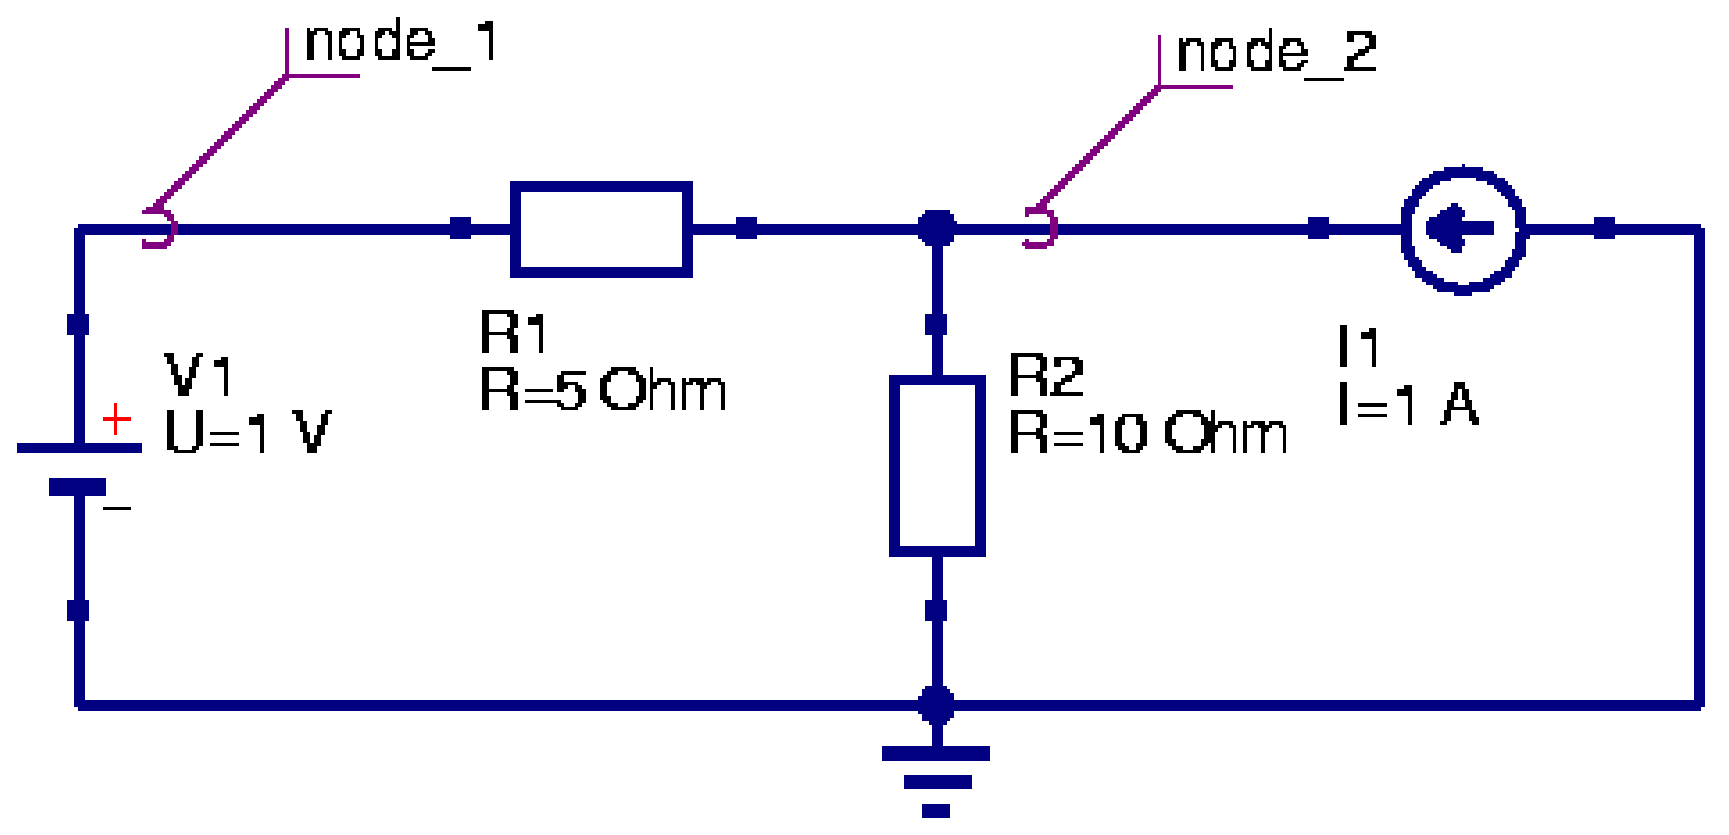
\includegraphics[angle=-90,width=10cm]{MNAexample}
\end{center}
\caption{example circuit applied to modified nodal analysis}
\label{fig:MNAexample}
\end{figure}
\FloatBarrier

\subsubsection{Going through the MNA algorithm}
%\addcontentsline{toc}{subsubsection}{Going through the MNA algorithm}

The G matrix is a 2$\times$2 matrix because there are 2 different
nodes apart from ground which is the reference node.  On the diagonal
you find the sum of the elements conductances connected to the nodes 1
and 2.  The off-diagonal matrix entries contain the negative
conductances of the elements connected between two nodes.

\begin{equation}
G =
\begin{bmatrix}
\frac{1}{R_{1}} & -\frac{1}{R_{1}}\\
-\frac{1}{R_{1}} & \frac{1}{R_{1}} + \frac{1}{R_{2}}
\end{bmatrix}
=
\begin{bmatrix}
0.2 & -0.2\\
-0.2 & 0.3
\end{bmatrix}
\end{equation}

The B matrix (which is transposed to C) is a 1$\times$2 matrix because
there is one voltage source and 2 nodes.  The positive terminal of the
voltage source $V_{1}$ is connected to node 1.  That is why

\begin{equation}
B = C^{T} =
\begin{bmatrix}
1\\
0
\end{bmatrix}
\end{equation}

and the D matrix is filled with zeros only because there are no dependent
(active and controlled) devices in the example circuit.

\begin{equation}
D =
\begin{bmatrix}
0
\end{bmatrix}
\end{equation}

The x matrix is a 1$\times$3 matrix.  The MNA equations deliver a
solution for the unknown voltages at each node in a circuit except the
reference node and the currents through each voltage source.

\begin{equation}
x =
\begin{bmatrix}
v_{1}\\
v_{2}\\
i_{V_{1}}
\end{bmatrix}
\end{equation}

The z matrix is according to the rules for building it a 1$\times$3
matrix.  The upper two entries are the sums of the currents flowing
into node 1 and node 2.  The lower entry is the voltage value of the
voltage source $V_{1}$.

\begin{equation}
z =
\begin{bmatrix}
0\\
I_{1}\\
U_{1}
\end{bmatrix}
=
\begin{bmatrix}
0\\
1\\
1
\end{bmatrix}
\end{equation}

According to the MNA algorithm the equation system is represented by

\begin{equation}
\left[A\right] \cdot \left[x\right] = \left[z\right]
\end{equation}

which is equivalent to

\begin{equation}
\begin{bmatrix}
G & B\\
C & D
\end{bmatrix}
\cdot
\begin{bmatrix}
x
\end{bmatrix}
=
\begin{bmatrix}
z
\end{bmatrix}
\label{eq:MNAexample}
\end{equation}

In the example eq. \eqref{eq:MNAexample} expands to:

\begin{equation}
\begin{bmatrix}
\frac{1}{R_{1}} & -\frac{1}{R_{1}} & 1\\
-\frac{1}{R_{1}} & \frac{1}{R_{1}} + \frac{1}{R_{2}} & 0\\
1 & 0 & 0
\end{bmatrix}
\cdot
\begin{bmatrix}
v_{1}\\
v_{2}\\
i_{V_{1}}
\end{bmatrix}
=
\begin{bmatrix}
0\\
I_{1}\\
U_{1}
\end{bmatrix}
\label{eq:MNAfull}
\end{equation}

The equation systems to be solved is now defined by the following
matrix representation.

\begin{equation}
\begin{bmatrix}
0.2 & -0.2 & 1\\
-0.2 & 0.3 & 0\\
1 & 0 & 0
\end{bmatrix}
\cdot
\begin{bmatrix}
v_{1}\\
v_{2}\\
i_{V_{1}}
\end{bmatrix}
=
\begin{bmatrix}
0\\
1\\
1
\end{bmatrix}
\end{equation}

Using matrix inversion the solution vector x writes as follows:

\begin{equation}
\left[x\right] = 
\left[A\right]^{-1}\cdot \left[z\right] = 
\begin{bmatrix}
v_{1}\\
v_{2}\\
i_{V_{1}}
\end{bmatrix}
=
\begin{bmatrix}
1\\
4\\
0.6
\end{bmatrix}
\label{eq:MNAresult}
\end{equation}

The result in eq. (\ref{eq:MNAresult}) denotes the current through the
voltage source $V_{1}$ is $0.6\ampere$, the voltage at node 1 is
$1\volt$ and the voltage at node 2 is $4\volt$.

\subsubsection{How the algorithm relates to basic equations in circuit analysis}
%\addcontentsline{toc}{subsubsection}{How the algorithm relates to basic equations in circuit analysis}

Expanding the matrix representation in eq. (\ref{eq:MNAfull}) to a set
of equations denotes the following equation system consisting of 3 of
them.

\begin{align}
\rm{I:}& \qquad 0 = \frac{1}{R_{1}}\cdot v_{1} - \frac{1}{R_{1}}\cdot v_{2} + i_{V_{1}}& \text{KCL at node 1}\\
\rm{II:}& \qquad I_{1} = -\frac{1}{R_{1}}\cdot v_{1} + \left(\frac{1}{R_{1}} + \frac{1}{R_{2}}\right)\cdot v_{2}& \text{KCL at node 2}\\
\rm{III:}& \qquad U_{1} = v_{1}& \text{constitutive equation}
\end{align}

Apparently eq. I and eq. II conform to Kirchhoff's current law at the
nodes 1 and 2.  The last equation is just the constitutive equation
for the voltage source $V_{1}$.  There are three unknowns ($v_{1}$,
$v_{2}$ and $i_{V_{1}}$) and three equations, thus the system should
be solvable.

\addvspace{12pt}

Equation III indicates the voltage at node 1 is $1\volt$.  Applying
this result to eq. II and transposing it to $v_{2}$ (the voltage at
node 2) gives

\begin{equation}
v_{2} = \frac{I_{1} + \frac{1}{R_{1}}\cdot U_{1}}{\frac{1}{R_{1}} + \frac{1}{R_{2}}} = 4\volt
\end{equation}

The missing current through the voltage source $V_{1}$ can be computed
using both the results $v_{2} = 4\volt$ and $v_{1} = 1\volt$ by
transforming equation I.

\begin{equation}
i_{V_{1}} = \frac{1}{R_{1}}\cdot v_{2} - \frac{1}{R_{1}}\cdot v_{1} = 0.6\ampere
\end{equation}

The small example, shown in fig. \ref{fig:MNAexample}, and the
excursus into artless math verifies that the MNA algorithm and classic
electrical handiwork tend to produce the same results.

\section{Solving linear equation systems}
%\addcontentsline{toc}{section}{Solving linear equation systems}

When dealing with non-linear networks the number of equation systems
to be solved depends on the required precision of the solution and the
average necessary iterations until the solution is stable.  This
emphasizes the meaning of the solving procedures choice for different
problems.

\addvspace{12pt}

The equation systems
\begin{equation}
\left[A\right] \cdot \left[x\right] = \left[z\right]
\end{equation}
solution can be written as
\begin{equation}
\left[x\right] = \left[A\right]^{-1} \cdot \left[z\right]
\end{equation}

\subsection{Matrix inversion}
%\addcontentsline{toc}{subsection}{Matrix inversion}

The elements $\beta_{\mu\nu}$ of the inverse of the matrix $A$ are
\begin{equation}
\beta_{\mu\nu} = \frac{A_{\mu\nu}}{det A}
\end{equation}
whereas $A_{\mu\nu}$ is the matrix elements $a_{\mu\nu}$ adjoint.  The
adjoint is the sub determinant of the element $a_{\mu\nu}$ multiplied
with $(-1)^{\mu + \nu}$.  The determinant of a square matrix can be
recursively computed by either of the following equations.
\begin{align}
det A = \sum_{\mu = 1}^{n} a_{\mu\nu}\cdot A_{\mu\nu}
\quad &\text{using the $\nu$-th column}\\
det A = \sum_{\nu = 1}^{n} a_{\mu\nu}\cdot A_{\mu\nu}
\quad &\text{using the $\mu$-th row}
\end{align}

This methode is called the Laplace expansion.  In order to save
computing time the row or column with the most zeros in it is used for
the expansion expressed in the above equations.  A sub determinant
$(n-1)$-th order of a matrix's element $a_{\mu\nu}$ of $n$-th order is
the determinant which is computed by canceling the $\mu$-th row and
$\nu$-th column.  The following example demonstrates calculating the
determinant of a 4th order matrix with the elements of the 3rd row.
\begin{align}
\begin{vmatrix}
a_{11} & a_{12} & a_{13} & a_{14}\\
a_{21} & a_{22} & a_{23} & a_{24}\\
a_{31} & a_{32} & a_{33} & a_{34}\\
a_{41} & a_{42} & a_{43} & a_{44}\\
\end{vmatrix}
&= a_{31}
\begin{vmatrix}
a_{12} & a_{13} & a_{14}\\
a_{22} & a_{23} & a_{24}\\
a_{42} & a_{43} & a_{44}\\
\end{vmatrix}
- a_{32}
\begin{vmatrix}
a_{11} & a_{13} & a_{14}\\
a_{21} & a_{23} & a_{24}\\
a_{41} & a_{43} & a_{44}\\
\end{vmatrix}\\
\nonumber
&+ a_{33}
\begin{vmatrix}
a_{11} & a_{12} & a_{14}\\
a_{21} & a_{22} & a_{24}\\
a_{41} & a_{42} & a_{44}\\
\end{vmatrix}
- a_{34}
\begin{vmatrix}
a_{11} & a_{12} & a_{13}\\
a_{21} & a_{22} & a_{23}\\
a_{41} & a_{42} & a_{43}\\
\end{vmatrix}
\end{align}

This recursive process for computing the inverse of a matrix is most
easiest to be implemented but as well the slowest algorithm.  It
requires approximately $n!$ operations.

\subsection{Gaussian elimination}
%\addcontentsline{toc}{subsection}{Gaussian elimination}

The Gaussian algorithm for solving a linear equation system is done in
two parts: forward elimination and backward substitution.  During
forward elimination the matrix A is transformed into an upper
triangular equivalent matrix.  Elementary transformations due to an
equation system having the same solutions for the unknowns as the
original system.

\begin{equation}
A =
\begin{bmatrix}
a_{11} & a_{12} & \ldots & a_{1n}\\
a_{21} & a_{22} & \ldots & a_{2n}\\
\vdots & \vdots & \ddots & \vdots\\
a_{n1} & a_{n2} & \ldots & a_{nn}
\end{bmatrix}
\rightarrow
\begin{bmatrix}
a_{11} & a_{12} & \ldots & a_{1n}\\
0 & a_{22} & \ldots & a_{2n}\\
\vdots & \vdots & \ddots & \vdots\\
0 & \ldots & 0 & a_{nn}
\end{bmatrix}
\end{equation}

The modifications applied to the matrix A in order to achieve this
transformations are limited to the following set of operations.
\begin{itemize}
\item multiplication of a row with a scalar factor
\item addition or subtraction of multiples of rows
\item exchanging two rows of a matrix
\end{itemize}

\subsubsection{Step 1: Forward elimination}
%\addcontentsline{toc}{subsubsection}{Step 1: Forward elimination}

The transformation of the matrix A is done in $\mathrm{n - 1}$
elimination steps.  The new matrix elements of the k-th step with
$\mathrm{k = 1, \ldots, n - 1}$ are computed with the following
recursive formulas.

\begin{align}
a_{ij} &= 0 & i = k+1, \ldots, n &\text{ and } j = k\\
a_{ij} &= a_{ij} - a_{kj} \cdot a_{ik} / a_{kk} & i = k+1, \ldots, n &\text{ and } j = k+1, \ldots, n\\
z_{i} &= z_{i} - z_{k} \cdot a_{ik} / a_{kk} & i = k+1, \ldots, n &
\end{align}

The triangulated matrix can be used to calculate the determinant very
easily.  The determinant of a triangulated matrix is the product of
the diagonal elements.  If the determinant $det A$ is non-zero the
equation system has a solution.  Otherwise the matrix A is singular.

\begin{equation}
det A = a_{11}\cdot a_{22}\cdot \ldots \cdot a_{nn} = \prod_{i=1}^{n} a_{ii}
\end{equation}

When using row and/or column pivoting the resulting determinant may
differ in its sign and must be multiplied with $(-1)^m$ whereas $m$ is
the number of row and column substitutions.

\subsubsection{Finding an appropriate pivot element}
%\addcontentsline{toc}{subsubsection}{Finding an appropriate pivot element}

The Gaussian elimination fails if the pivot element $a_{kk}$ turns to
be zero (division by zero).  That is why row and/or column pivoting
must be used before each elimination step.  If a diagonal element
$a_{kk} = 0$, then exchange the pivot row $k$ with the row $m > k$
having the coefficient with the largest absolute value.  The new pivot
row is $m$ and the new pivot element is going to be $a_{mk}$.  If no
such pivot row can be found the matrix is singular.

\addvspace{12pt}

Total pivoting looks for the element with the largest absolute value
within the matrix and exchanges rows and columns.  When exchanging
columns in equation systems the unknowns get reordered as well.  For
the numerical solution of equation systems with Gaussian elimination
column pivoting is clever, and total pivoting recommended.

\addvspace{12pt}

In order to improve numerical stability pivoting should also be
applied if $a_{kk} \ne 0$ because division by small diagonal elements
propagates numerical (rounding) errors.  This appears especially with
poorly conditioned (the two dimensional case: two lines with nearly
the same slope) equation systems.

\subsubsection{Step 2: Backward substitution}
%\addcontentsline{toc}{subsubsection}{Step 2: Backward substitution}

The solutions in the vector x are obtained by backward substituting
into the triangulated matrix.  The elements of the solution vector x
are computed by the following recursive equations.

\begin{align}
x_{n} &= \frac{z_{n}}{a_{nn}}\\
x_{i} &= \frac{z_{i}}{a_{ii}} - \sum_{k=i+1}^{n} x_{k}\cdot \frac{a_{ik}}{a_{ii}} & i = n - 1,\ldots,1
\end{align}

The forward elimination in the Gaussian algorithm requires
approximately $n^3/3$, the backward substitution $n^2/2$ operations.

\subsection{LU decomposition}
%\addcontentsline{toc}{subsection}{LU decomposition}

LU decomposition (decomposition into a lower and upper triangular
matrix) is recommended when dealing with equation systems where the
matrix A does not alter but the right hand side (the vector z) does.
Both the Gaussian elimination and the Gauss-Jordan method involve both
the right hand side and the matrix in their algorithm.  Consecutive
solutions of an equation system with an altering right hand side can
be computed faster with LU decomposition.

\addvspace{12pt}

The LU decomposition splits a matrix A into a product of a lower
triangular matrix L with an upper triangular matrix U.

\begin{equation}
A = L U \;\text{ with }\;
L = 
\begin{bmatrix}
l_{11} & 0 & \ldots & 0\\
l_{21} & l_{22} & \ddots & \vdots\\
\vdots &  & \ddots & 0\\
l_{n1} & \ldots & \ldots & l_{nn}
\end{bmatrix}
\;\text{ and }\;
U =
\begin{bmatrix}
u_{11} & u_{12} & \ldots & u_{1n}\\
0 & u_{22} &  & \vdots\\
\vdots & \ddots & \ddots & \vdots\\
0 & \ldots & 0 & u_{nn}
\end{bmatrix}
\end{equation}

The algorithm for solving the linear equation system $Ax = z$ involves
three steps:
\begin{itemize}
\item LU decomposition of the coefficient matrix A\\
$\rightarrow Ax = LUx = z$
\item introduction of an (unknown) arbitrary vector y and solving the equation system $Ly = z$ by forward substitution\\
$\rightarrow y = Ux = L^{-1}z$
\item solving the equation system $Ux = y$  by backward substitution\\
$\rightarrow x = U^{-1}y$
\end{itemize}

The decomposition of the matrix A into a lower and upper triangular
matrix is not unique.  The most important decompositions, based on
Gaussian elimination, are the Doolittle, the Crout and the Cholesky
decomposition.

\addvspace{12pt}

If pivoting is necessary during these algorithms they do not decompose
the matrix $A$ but the product with an arbitrary matrix $PA$ (a
permutation of the matrix $A$).  When exchanging rows and columns the
order of the unknowns as represented by the vector $z$ changes as well
and must be saved during this process for the forward substitution in
the algorithms second step.

\subsubsection{Step 1: LU decomposition}
%\addcontentsline{toc}{subsubsection}{Step 1: LU decomposition}

Using the decomposition according to Crout the coefficients of the L
and U matrices can be stored in place the original matrix A.  The
upper triangular matrix U has the form

\begin{equation}
U = 
\begin{bmatrix}
1 & u_{12} & \ldots & u_{1n}\\
0 & 1 &  & \vdots\\
\vdots & \ddots & \ddots & u_{n-1,n}\\
0 & \ldots & 0 & 1
\end{bmatrix}
\label{eq:CroutU}
\end{equation}

The diagonal elements $u_{jj}$ are ones and thus the determinant $det
U$ is one as well.  The elements of the new coefficient matrix $LU$
for the k-th elimination step with $k = 1, \ldots,n$ compute as
follows:
\begin{align}
u_{jk} &= \frac{1}{l_{jj}}\left(a_{jk} - \sum_{r=1}^{j-1} l_{jr} u_{rk}\right) & j &= 1,\ldots,k-1\\
l_{jk} &= a_{jk} - \sum_{r=1}^{k-1} l_{jr} u_{rk} & j &= k,\ldots,n
\end{align}

Pivoting may be necessary as you are going to divide by the diagonal
element $l_{jj}$.

\subsubsection{Step 2: Forward substitution}
%\addcontentsline{toc}{subsubsection}{Step 2: Forward substitution}

The solutions in the arbitrary vector $y$ are obtained by forward
substituting into the triangulated $L$ matrix.  At this stage you need
to remember the order of unknowns in the vector $z$ as changed by
pivoting.  The elements of the solution vector $y$ are computed by the
following recursive equation.

\begin{align}
y_{i} &= \frac{z_{i}}{l_{ii}} - \sum_{k=1}^{i-1} y_{k}\cdot \frac{l_{ik}}{l_{ii}} & i = 1,\ldots,n
\end{align}

\subsubsection{Step 3: Backward substitution}
%\addcontentsline{toc}{subsubsection}{Step 3: Backward substitution}

The solutions in the vector $x$ are obtained by backward substituting
into the triangulated $U$ matrix.  The elements of the solution vector
$x$ are computed by the following recursive equation.

\begin{align}
x_{i} &= y_{i} - \sum_{k=i+1}^{n} x_{k}\cdot u_{ik} & i = n,\ldots,1
\end{align}

The division by the diagonal elements of the matrix U is not necessary
because of Crouts definition in eq. (\ref{eq:CroutU}) with $u_{ii} =
1$.

\addvspace{12pt}

The LU decomposition requires approximately $n^3/3 + n^2 - n/3$
operations for solving a linear equation system.  For $M$ consecutive
solutions the method requires $n^3/3 + Mn^2 - n/3$ operations.

\subsection{A comparison}
%\addcontentsline{toc}{subsection}{A comparison}

There are direct and iterative methods (algorithms) for solving linear
equation systems.  Equation systems with large and sparse matrices
should rather be solved with iterative methods.

\addvspace{12pt}

\begin{tabular}{|p{2.2cm}|p{1.5cm}|p{1.8cm}|p{2.1cm}|p{1.7cm}|p{2.95cm}|}
\hline
\raggedright method & \raggedleft precision & \raggedleft application & 
\raggedleft programming effort & \raggedleft computing complexity & 
\parbox[t]{2.95cm}{\raggedleft notes}\\
\hline
\raggedright Laplace expansion & \raggedleft numerical errors & 
\raggedleft general & \raggedleft straight forward &
\raggedleft $n!$ & \parbox[t]{2.95cm}{\raggedleft very time consuming}\\
\hline
\raggedright Gaussian elimination & \raggedleft numerical errors & 
\raggedleft general & \raggedleft intermediate & \raggedleft $n^3/3 + n^2/2$ &
\parbox[t]{2.95cm}{\raggedleft }\\
\hline
\raggedright Gauss-Jordan & \raggedleft numerical errors & \raggedleft general & \raggedleft intermediate & \raggedleft $n^3/3 + n^2 - n/3$ & \parbox[t]{2.95cm}{\raggedleft computes the inverse besides}\\
\hline
\raggedright LU decomposition & \raggedleft numerical errors & \raggedleft general & \raggedleft intermediate & \raggedleft $n^3/3 + n^2 - n/3$ & \parbox[t]{2.95cm}{\raggedleft useful for consecutive solutions}

\addvspace{1pt}

\\
\hline
\raggedright Jacobi & \raggedleft ? & \raggedleft ? & \raggedleft ? & \raggedleft ? & \parbox[t]{2.95cm}{\raggedleft }\\
\hline
\raggedright Gauss-Seidel & \raggedleft very good & \raggedleft diagonally dominant systems & \raggedleft easy & & \parbox[t]{2.95cm}{\raggedleft possibly no convergence}\\
\hline
\end{tabular}

\section{Extensions to the MNA}
%\addcontentsline{toc}{section}{Extensions to the MNA}

As noted in the previous sections the D matrix is zero and the B and C
matrices are transposed each other and filled with either 1, -1 or 0
provided that there are no dependent sources within the circuit.  This
changes when introducing active (and controlled) elements.

\subsection{Voltage controlled current source}
%\addcontentsline{toc}{subsection}{Voltage controlled current source}

The voltage-dependent current source (VCCS), as shown in fig.
\ref{fig:vccs}, is determined by the following equation which
introduces one more unknown in the MNA matrix.

\begin{figure}[ht]
\begin{center}
\includegraphics[width=4cm]{vccs}
\end{center}
\caption{voltage controlled current source}
\label{fig:vccs}
\end{figure}
\FloatBarrier

\begin{equation}
I_{out} = G\cdot\left(V_{1} - V_{2}\right)
\quad \rightarrow \quad
V_{1} - V_{4} - \frac{1}{G}\cdot I_{out} = 0
\label{eq:vccs}
\end{equation}

The new unknown variable $I_{out}$ must be considered by the four
remaining simple equations.

\begin{equation}
I_{1} = 0 \quad I_{2} = I_{out} \quad I_{3} = -I_{out} \quad I_{4} = 0
\end{equation}

And in matrix representation this is:
\begin{equation}
\begin{bmatrix}
.&.&.&.& 0\\
.&.&.&.& 1\\
.&.&.&.& -1\\
.&.&.&.& 0\\
1 & 0 & 0 & -1 & -\frac{1}{G}
\end{bmatrix}
\cdot
\begin{bmatrix}
V_{1}\\
V_{2}\\
V_{3}\\
V_{4}\\
I_{out}\\
\end{bmatrix}
=
\begin{bmatrix}
I_{1}\\
I_{2}\\
I_{3}\\
I_{4}\\
0\\
\end{bmatrix}
\end{equation}

As you can see the last row which has been added by the VCCS
represents the determining equation (\ref{eq:vccs}).  The additional
right hand column in the matrix keeps the system consistent.

\subsection{Voltage controlled voltage source}
%\addcontentsline{toc}{subsection}{Voltage controlled voltage source}

The voltage-dependent voltage source (VCVS), as shown in fig.
\ref{fig:vcvs}, is determined by the following equation which
introduces one more unknown in the MNA matrix.

\begin{figure}[ht]
\begin{center}
\includegraphics[width=4cm]{vcvs}
\end{center}
\caption{voltage controlled voltage source}
\label{fig:vcvs}
\end{figure}
\FloatBarrier

\begin{equation}
V_{2} - V_{3} = G\cdot \left(V_{1} - V_{4}\right)
\quad \rightarrow \quad
V_{1}\cdot G - V_{2} + V_{3} - V_{4}\cdot G = 0
\label{eq:vcvs}
\end{equation}

The new unknown variable $I_{out}$ must be considered by the four
remaining simple equations.

\begin{equation}
I_{1} = 0 \quad I_{2} = -I_{out} \quad I_{3} = I_{out} \quad I_{4} = 0
\end{equation}

And in matrix representation this is:
\begin{equation}
\begin{bmatrix}
.&.&.&.& 0\\
.&.&.&.& -1\\
.&.&.&.& 1\\
.&.&.&.& 0\\
G & -1 & 1 & -G & 0
\end{bmatrix}
\cdot
\begin{bmatrix}
V_{1}\\
V_{2}\\
V_{3}\\
V_{4}\\
I_{out}\\
\end{bmatrix}
=
\begin{bmatrix}
I_{1}\\
I_{2}\\
I_{3}\\
I_{4}\\
0\\
\end{bmatrix}
\end{equation}

\subsection{Current controlled current source}
%\addcontentsline{toc}{subsection}{Current controlled current source}

The current-dependent current source (CCCS), as shown in fig.
\ref{fig:cccs}, is determined by the following equation which
introduces one more unknown in the MNA matrix.

\begin{figure}[ht]
\begin{center}
\includegraphics[width=4cm]{cccs}
\end{center}
\caption{current controlled current source}
\label{fig:cccs}
\end{figure}
\FloatBarrier

\begin{equation}
V_{1} - V_{4} = 0
\label{eq:cccs}
\end{equation}

The new unknown variable $I_{out}$ must be considered by the four
remaining simple equations.

\begin{equation}
I_{1} = +\frac{1}{G}\cdot I_{out} \quad I_{2} = I_{out} \quad I_{3} = -I_{out} \quad I_{4} = -\frac{1}{G}\cdot I_{out}
\end{equation}

And in matrix representation this is:
\begin{equation}
\begin{bmatrix}
.&.&.&.& \frac{1}{G}\\
.&.&.&.& 1\\
.&.&.&.& -1\\
.&.&.&.& -\frac{1}{G}\\
1 & 0 & 0 & -1 & 0
\end{bmatrix}
\cdot
\begin{bmatrix}
V_{1}\\
V_{2}\\
V_{3}\\
V_{4}\\
I_{out}\\
\end{bmatrix}
=
\begin{bmatrix}
I_{1}\\
I_{2}\\
I_{3}\\
I_{4}\\
0\\
\end{bmatrix}
\end{equation}

\subsection{Current controlled voltage source}
%\addcontentsline{toc}{subsection}{Current controlled voltage source}

The current-dependent voltage source (CCVS), as shown in fig.
\ref{fig:ccvs}, is determined by the following equations which
introduce two more unknowns in the MNA matrix.

\begin{figure}[ht]
\begin{center}
\includegraphics[width=4cm]{ccvs}
\end{center}
\caption{current controlled voltage source}
\label{fig:ccvs}
\end{figure}
\FloatBarrier

\begin{equation}
V_{1} - V_{4} = 0
\end{equation}
\begin{equation}
V_{2} - V_{3} = G\cdot I_{in}
\quad \rightarrow \quad
V_{2} - V_{3} - I_{in}\cdot G = 0
\label{eq:ccvs}
\end{equation}

The new unknown variables $I_{out}$ and $I_{in}$ must be considered by
the four remaining simple equations.

\begin{equation}
I_{1} = I_{in} \quad I_{2} = -I_{out} \quad I_{3} = I_{out} \quad I_{4} = -I_{in}
\end{equation}

The matrix representation needs to be augmented by two more new rows
(for the new unknown variables) and their corresponding columns.
\begin{equation}
\begin{bmatrix}
.&.&.&.& 1 & 0\\
.&.&.&.& 0 & -1\\
.&.&.&.& 0 & 1\\
.&.&.&.& -1 & 0\\
0 & 1 & -1 & 0 & -G & 0\\
1 & 0 & 0 & -1 & 0 & 0
\end{bmatrix}
\cdot
\begin{bmatrix}
V_{1}\\
V_{2}\\
V_{3}\\
V_{4}\\
I_{in}\\
I_{out}
\end{bmatrix}
=
\begin{bmatrix}
I_{1}\\
I_{2}\\
I_{3}\\
I_{4}\\
0\\
0
\end{bmatrix}
\end{equation}

\subsection{Operational amplifier}
%\addcontentsline{toc}{subsection}{Operational amplifier}

The ideal operational amplifier, as shown in fig. \ref{fig:opamp}, is
determined by the following equation which introduces one more unknown
in the MNA matrix.

\begin{figure}[ht]
\begin{center}
\includegraphics[width=4cm]{opamp}
\end{center}
\caption{ideal operational amplifier}
\label{fig:opamp}
\end{figure}
\FloatBarrier

\begin{equation}
V_{1} - V_{3} = 0
\label{eq:opamp}
\end{equation}

The new unknown variable $I_{out}$ must be considered by the three
remaining simple equations.

\begin{equation}
I_{1} = 0 \quad I_{2} = I_{out} \quad I_{3} = 0
\end{equation}

And in matrix representation this is:
\begin{equation}
\begin{bmatrix}
.&.&.& 0\\
.&.&.& 1\\
.&.&.& 0\\
1 & 0 & -1 & 0
\end{bmatrix}
\cdot
\begin{bmatrix}
V_{1}\\
V_{2}\\
V_{3}\\
I_{out}
\end{bmatrix}
=
\begin{bmatrix}
I_{1}\\
I_{2}\\
I_{3}\\
0
\end{bmatrix}
\end{equation}

The operational amplifier could be considered as a special case of a
voltage controlled current source with infinite forward
transconductance $G$.  Please note that the presented matrix form is
only valid in case there is any kind of finite feedback impedance
between the output and input port.

\subsection{Transformer}
%\addcontentsline{toc}{subsection}{Transformer}

The two winding ideal transformer, as shown in fig.
\ref{fig:actrafo}, is determined by the following equation which
introduces one more unknown in the MNA matrix.

\begin{figure}[ht]
\begin{center}
\includegraphics[width=4cm]{actrafo}
\end{center}
\caption{ideal two winding transformer}
\label{fig:actrafo}
\end{figure}
\FloatBarrier

\begin{equation}
T\cdot\left(V_{2} - V_{3}\right) = V_{1} -V_{4}
\quad \rightarrow \quad
V_{1} - T\cdot V_{2} + T\cdot V_{3} - V_{4} = 0
\label{eq:trafo}
\end{equation}

The new unknown variable $I_{t}$ must be considered by the four
remaining simple equations.

\begin{equation}
I_{1} = -I_{t} \quad I_{2} = T\cdot I_{t} \quad I_{3} = -T\cdot I_{t} \quad I_{4} = I_{t}
\end{equation}

And in matrix representation this is:
\begin{equation}
\begin{bmatrix}
.&.&.&.& -1\\
.&.&.&.& T\\
.&.&.&.& -T\\
.&.&.&.& 1\\
1 & -T & T & -1 & 0
\end{bmatrix}
\cdot
\begin{bmatrix}
V_{1}\\
V_{2}\\
V_{3}\\
V_{4}\\
I_{t}
\end{bmatrix}
=
\begin{bmatrix}
I_{1}\\
I_{2}\\
I_{3}\\
I_{4}\\
0
\end{bmatrix}
\end{equation}

It is noticeable that the additional row (part of the C matrix) and the
corresponding column (part of the B matrix) are transposed to each
other.  When considering the turns ratio $T$ being complex introducing
an additional phase the transformer can be used as phase-shifting
transformer.  Both the vectors must be conjugated complex transposed
in this case.

\subsection{Symmetrical transformer}
%\addcontentsline{toc}{subsection}{Symmetrical transformer}

The ideal symmetrical transformer, as shown in fig.
\ref{fig:acstrafo}, is determined by the following equations which
introduce two more unknowns in the MNA matrix.

\begin{figure}[ht]
\begin{center}
\includegraphics[width=4cm]{acstrafo}
\end{center}
\caption{ideal three winding transformer}
\label{fig:acstrafo}
\end{figure}
\FloatBarrier

\begin{equation}
T_{1}\cdot\left(V_{2} - V_{3}\right) = V_{1} - V_{6}
\quad \rightarrow \quad
V_{1} - T_{1}\cdot V_{2} + T_{1}\cdot V_{3} - V_{6} = 0
\end{equation}
\begin{equation}
T_{2}\cdot\left(V_{2} - V_{3}\right) = V_{5} - V_{4}
\quad \rightarrow \quad
- T_{2}\cdot V_{2} + T_{2}\cdot V_{3} - V_{4} + V_{5} = 0
\label{eq:acstrafo}
\end{equation}

The new unknown variables $I_{T1}$ and $I_{T2}$ must be considered by
the eight remaining simple equations.

\begin{equation}
I_{1} = -I_{T1} \quad I_{2} = T_{1}\cdot I_{T1} \quad I_{3} = -T_{1}\cdot I_{T1} \quad I_{6} = I_{T1}
\end{equation}
\begin{equation}
I_{2} = T_{2}\cdot I_{T2} \quad I_{3} = -T_{2}\cdot I_{T2} \quad I_{4} = I_{T2} \quad I_{5} = -I_{T2}
\end{equation}

The matrix representation needs to be augmented by two more new rows
and their corresponding columns.
\begin{equation}
\begin{bmatrix}
.&.&.&.&.&.& -1 & 0\\
.&.&.&.&.&.& T_{1} & T_{2}\\
.&.&.&.&.&.& -T_{1} & -T_{2}\\
.&.&.&.&.&.& 0 & 1\\
.&.&.&.&.&.& 0 & -1\\
.&.&.&.&.&.& 1 & 0\\
1 & -T_{1} & T_{1} & 0 & 0 & -1 & 0 & 0\\
0 & -T_{2} & T_{2} & -1 & 1 & 0 & 0 & 0
\end{bmatrix}
\cdot
\begin{bmatrix}
V_{1}\\
V_{2}\\
V_{3}\\
V_{4}\\
V_{5}\\
V_{6}\\
I_{T1}\\
I_{T2}
\end{bmatrix}
=
\begin{bmatrix}
I_{1}\\
I_{2}\\
I_{3}\\
I_{4}\\
I_{5}\\
I_{6}\\
0\\
0
\end{bmatrix}
\end{equation}

\subsection{Gyrator}
%\addcontentsline{toc}{subsection}{Gyrator}

The ideal gyrator, as shown in fig. \ref{fig:gyrator}, is determined
by the following equations which introduce two more unknowns in the
MNA matrix.

\begin{figure}[ht]
\begin{center}
\includegraphics[width=4cm]{gyrator}
\end{center}
\caption{ideal gyrator}
\label{fig:gyrator}
\end{figure}
\FloatBarrier

\begin{equation}
I_{in} = \frac{1}{R}\cdot\left(V_{2} - V_{3}\right)
\quad \rightarrow \quad
\frac{1}{R}\cdot V_{2} - \frac{1}{R}\cdot V_{3} - I_{in} = 0
\end{equation}
\begin{equation}
I_{out} = -\frac{1}{R}\cdot\left(V_{1} - V_{4}\right)
\quad \rightarrow \quad
-\frac{1}{R}\cdot V_{1} + \frac{1}{R}\cdot V_{4} - I_{out} = 0
\label{eq:gyrator}
\end{equation}

The new unknown variables $I_{out}$ and $I_{in}$ must be considered by
the four remaining simple equations.

\begin{equation}
I_{1} = I_{in} \quad I_{2} = I_{out} \quad I_{3} = -I_{out} \quad I_{4} = -I_{in}
\end{equation}

The matrix representation needs to be augmented by two more new rows
(for the new unknown variables) and their corresponding columns.
\begin{equation}
\begin{bmatrix}
.&.&.&.& 1 & 0\\
.&.&.&.& 0 & 1\\
.&.&.&.& 0 & -1\\
.&.&.&.& -1 & 0\\
0 & \frac{1}{R} & -\frac{1}{R} & 0 & -1 & 0\\
-\frac{1}{R} & 0 & 0 & \frac{1}{R} & 0 & -1
\end{bmatrix}
\cdot
\begin{bmatrix}
V_{1}\\
V_{2}\\
V_{3}\\
V_{4}\\
I_{in}\\
I_{out}
\end{bmatrix}
=
\begin{bmatrix}
I_{1}\\
I_{2}\\
I_{3}\\
I_{4}\\
0\\
0
\end{bmatrix}
\end{equation}

\subsection{Attenuator}
%\addcontentsline{toc}{subsection}{Attenuator}

The ideal attenuator with (power) attenuation $L$ is determined by the
following Z parameters.

\begin{equation}
Z_{11} = Z_{22} = Z_{ref}\cdot\frac{L+1}{L-1}
\end{equation}
\begin{equation}
Z_{12} = Z_{21} = Z_{ref}\cdot\frac{2\cdot\sqrt{L}}{L-1}
\end{equation}

The MNA matrix representation can be derived from the Z parameters in the
following way.
\begin{equation}
\begin{bmatrix}
 . & .  &  1 & 0\\
 . & .  &  0 & 1\\
-1 &  0 & Z_{11} & Z_{12}\\
 0 & -1 & Z_{21} & Z_{22}
\end{bmatrix}
\cdot
\begin{bmatrix}
V_{1}\\
V_{2}\\
I_{in}\\
I_{out}
\end{bmatrix}
=
\begin{bmatrix}
I_{1}\\
I_{2}\\
0\\
0
\end{bmatrix}
\end{equation}


\subsection{Isolator}
%\addcontentsline{toc}{subsection}{Isolator}

The ideal isolator with reference impedances $Z_1$ (input) and $Z_2$
(output) is determined by the following Z parameters.

\begin{equation}
Z_{11} = Z_1  \qquad
Z_{12} = 0
\end{equation}
\begin{equation}
Z_{21} = 2\cdot\sqrt{Z_1\cdot Z_2}  \qquad
Z_{22} = Z_2
\end{equation}

The MNA matrix representation can be derived from the Z parameters in the
following way.
\begin{equation}
\begin{bmatrix}
 . & .  &  1 & 0\\
 . & .  &  0 & 1\\
-1 &  0 & Z_{11} & Z_{12}\\
 0 & -1 & Z_{21} & Z_{22}
\end{bmatrix}
\cdot
\begin{bmatrix}
V_{1}\\
V_{2}\\
I_{in}\\
I_{out}
\end{bmatrix}
=
\begin{bmatrix}
I_{1}\\
I_{2}\\
0\\
0
\end{bmatrix}
\end{equation}


\subsection{Phase Shifter}

A phase shifter alters the phase of the input signal independently on
the frequency.  As a result the relation between input and output
signal is complex.  To get the DC model, some simulators use the AC
formulas and create the real part or the magnitude.  This procedure
has no physical reason, because it uses an operation that is not
defined for DC.  But one can think in the following direction: As a DC
quantity is constant, it doesn't change if it is phase-shifted.  (An
AC quantity doesn't change it magnitude, too.)  Or to say it with
other words, for a DC simulation the phase to shift is always zero.
That leads to the result that the phase shifter is a short circuit for
DC.  So, this is true for all reference impedances.

\subsection{Circulator}
%\addcontentsline{toc}{subsection}{Circulator}

The ideal circulator cannot be characterized with Z or Y parameters,
because their values are partly infinite.  But implementing with S
parameters is practical (see chapter \ref{sec:CirculatorSparameter}
for S parameters of the circulator).
\begin{equation}
\begin{bmatrix}
 . & . & .  &  1 & 0 & 0\\
 . & . & .  &  0 & 1 & 0\\
 . & . & .  &  0 & 0 & 1\\
S_{11}-1 &  S_{12} & S_{13} & Z_0\cdot (S_{11}+1) & Z_0\cdot S_{12} & Z_0\cdot S_{13}\\
S_{21} &  S_{22}-1 & S_{23} & Z_0\cdot S_{21} & Z_0\cdot (S_{22}+1) & Z_0\cdot S_{23}\\
S_{31} &  S_{32} & S_{33}-1 & Z_0\cdot S_{31} & Z_0\cdot S_{32} & Z_0\cdot (S_{33}+1)
\end{bmatrix}
\cdot
\begin{bmatrix}
V_{1}\\
V_{2}\\
V_{3}\\
I_{I1}\\
I_{I2}\\
I_{I3}
\end{bmatrix}
=
\begin{bmatrix}
I_{1}\\
I_{2}\\
I_{3}\\
0\\
0\\
0
\end{bmatrix}
\end{equation}

\subsection{Bias T}
%\addcontentsline{toc}{subsection}{Bias T}

The MNA matrix of an ideal bias t (with ports as shown in
fig. \ref{fig:biast}) writes as follows:
\begin{equation}
\begin{bmatrix}
 . & . & .  &  0\\
 . & . & .  &  1\\
 . & . & .  & -1\\
 0 & 1 & -1 &  0
\end{bmatrix}
\cdot
\begin{bmatrix}
V_{1}\\
V_{2}\\
V_{3}\\
I_{out}
\end{bmatrix}
=
\begin{bmatrix}
I_{1}\\
I_{2}\\
I_{3}\\
0
\end{bmatrix}
\end{equation}

\section{Non-linear DC Analysis}
%\addcontentsline{toc}{section}{Non-linear DC Analysis}

Previous sections described using the modified nodal analysis solving
linear networks including controlled sources.  It can also be used to
solve networks with non-linear components like diodes and transistors.
Most methods are based on iterative solutions of a linearised equation
system.  The best known is the so called Newton-Raphson method.

\subsection{Newton-Raphson method}
%\addcontentsline{toc}{subsection}{Newton-Raphson method}

The Newton-Raphson method is going to be introduced using the example
circuit shown in fig. \ref{fig:NLexample} having a single unknown: the
voltage at node 1.

\begin{figure}[ht]
\begin{center}
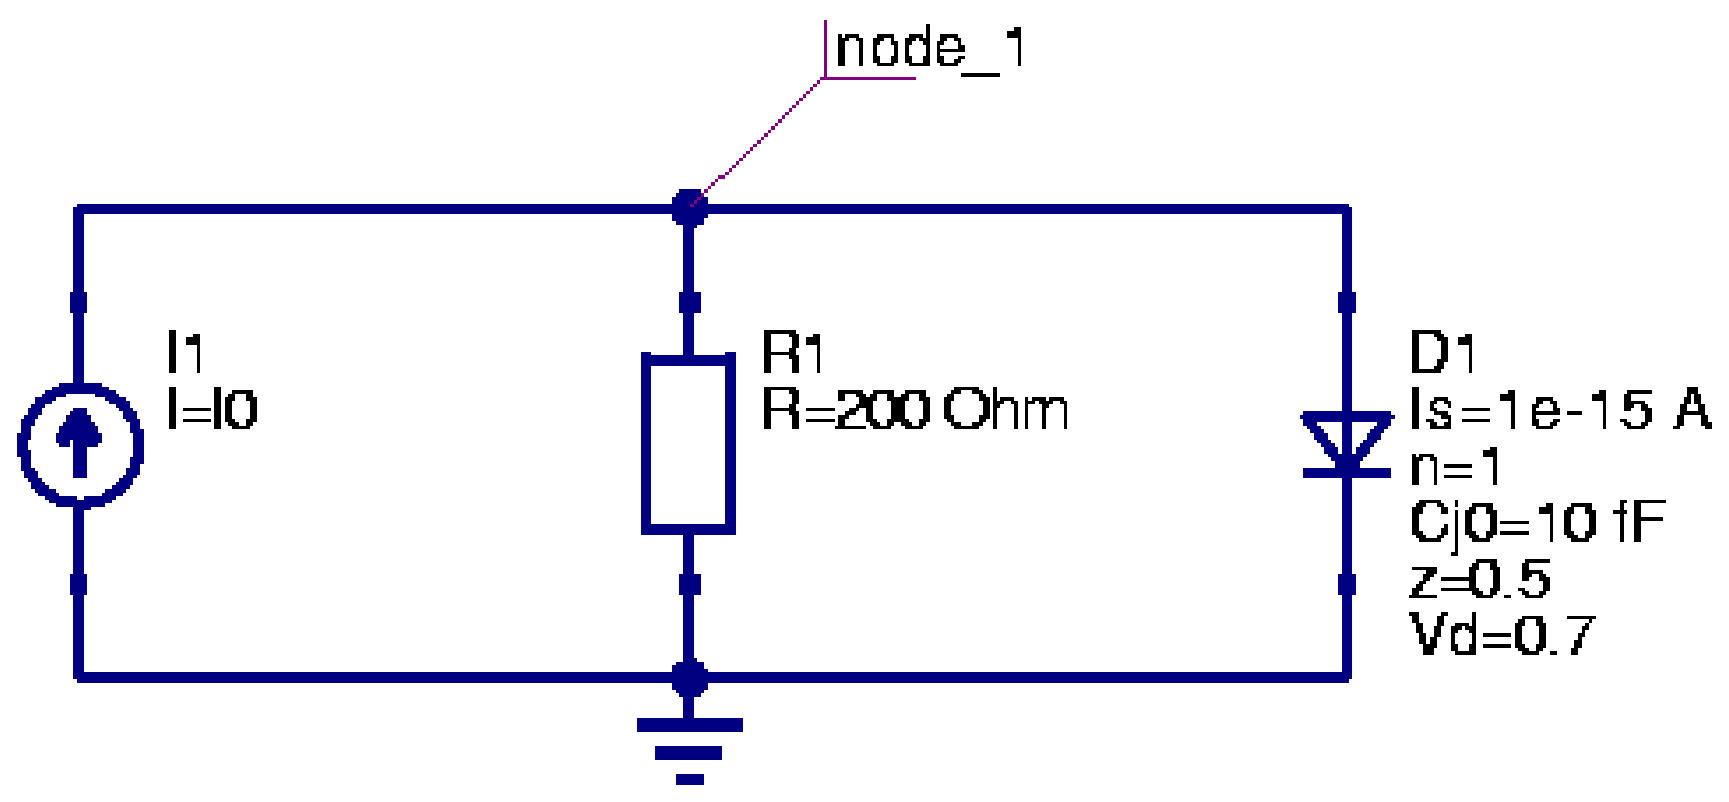
\includegraphics[angle=-90,width=10cm]{NLexample}
\end{center}
\caption{example circuit for non-linear DC analysis}
\label{fig:NLexample}
\end{figure}
\FloatBarrier

The 1x1 MNA equation system to be solved can be written as
\begin{equation}
\begin{bmatrix}
G
\end{bmatrix}
\cdot
\begin{bmatrix}
V_{1}
\end{bmatrix}
=
\begin{bmatrix}
I_{0}
\end{bmatrix}
\label{eq:NLmatrix}
\end{equation}

whereas the value for $G$ is now going to be explained.  The current
through a diode is simply determined by Schockley's approximation
\begin{equation}
I_{d} = I_{S}\cdot \left(e^{\frac{V_{d}}{V_{T}}} - 1\right)
\end{equation}

Thus Kirchhoff's current law at node 1 can be expressed as
\begin{equation}
I_{0} = \dfrac{V}{R} + I_{S}\cdot \left(e^{\frac{V}{V_{T}}} - 1\right)
\end{equation}

By establishing eq. (\ref{eq:NLfunc}) it is possible to trace the
problem back to finding the zero point of the function $f$.
\begin{equation}
f(V) = \dfrac{V}{R} + I_{S}\cdot \left(e^{\frac{V}{V_{T}}} - 1\right) - I_{0}
\label{eq:NLfunc}
\end{equation}

Newton developed a method stating that the zero point of a functions
derivative (i.e. the tangent) at a given point is nearer to the zero
point of the function itself than the original point.  In mathematical
terms this means to linearise the function $f$ at a starting value
$V^{(0)}$.
\begin{equation}
f\left(V^{(0)} + \Delta V\right) \approx f\left(V^{(0)}\right) + \left.\dfrac{\partial f\left(V\right)}{\partial V}\right|_{V^{(0)}}\cdot \Delta V
\;\;\;\; \text{ with } \;\;\;\;
\Delta V = V^{(1)} - V^{(0)}
\label{eq:NRapprox}
\end{equation}

Setting $f(V^{(1)}) = 0$ gives
\begin{equation}
V^{(1)} = V^{(0)} - \dfrac{f\left(V^{(0)}\right)}{\left.\dfrac{\partial f\left(V\right)}{\partial V}\right|_{V^{(0)}}}
\end{equation}

or in the general case with $m$ being the number of iteration
\begin{equation}
V^{(m + 1)} = V^{(m)} - \dfrac{f\left(V^{(m)}\right)}{\left.\dfrac{\partial f\left(V\right)}{\partial V}\right|_{V^{(m)}}}
\label{eq:NRgeneral}
\end{equation}

This must be computed until $V^{(m+1)}$ and $V^{(m)}$ differ less than a
certain barrier.
\begin{equation}
\left|V^{(m+1)} - V^{(m)}\right| < \varepsilon_{abs} + \varepsilon_{rel}\cdot \left|V^{(m)}\right|
\label{eq:NLconvergence}
\end{equation}

With very small $\varepsilon_{abs}$ the iteration would break too
early and for little $\varepsilon_{rel}$ values the iteration aims to
a useless precision for large absolute values of $V$.

\begin{figure}[ht]
\begin{center}
\psfrag{V0}{$\mathrm{V^{(0)}}$}
\psfrag{V1}{$\mathrm{V^{(1)}}$}
\psfrag{V2}{$\mathrm{V^{(2)}}$}
\includegraphics[width=0.75\linewidth]{newton}
\end{center}
\caption{Newton-Raphson method for example circuit}
\label{fig:NewtonRaphson}
\end{figure}
\FloatBarrier

With this theoretical background it is now possible to step back to
eq. (\ref{eq:NLfunc}) being the determining equation for the example
circuit.  With
\begin{equation}
g_{d}^{(m)} = \left.\dfrac{\partial I_{d}}{\partial V}\right|_{V^{(m)}} = \dfrac{I_{S}}{V_{T}}\cdot e^{\frac{V^{(m)}}{V_{T}}}
\end{equation}

and
\begin{equation}
\left.\dfrac{\partial f\left(V\right)}{\partial V}\right|_{V^{(m)}} = \dfrac{1}{R} + g_{d}^{(m)}
\end{equation}

the eq. (\ref{eq:NRgeneral}) can be written as
\begin{equation}
\left(g_{d}^{(m)} + \dfrac{1}{R}\right)\cdot V^{(m+1)} = I_{0} - \left(I_{d}^{(m)} - g_{d}^{(m)}\cdot V^{(m)}\right)
\label{eq:NRresult}
\end{equation}

when the expression
\begin{equation}
f\left(V^{(m)}\right) = \dfrac{1}{R}\cdot V^{(m)} + I_{d}^{(m)} - I_{0}
\end{equation}

based upon eq. (\ref{eq:NLfunc}) is taken into account.  Comparing the
introductory MNA equation system in eq. (\ref{eq:NLmatrix}) with
eq. (\ref{eq:NRresult}) proposes the following equivalent circuit for
the diode model.

\begin{figure}[ht]
\begin{center}
\psfrag{gd}{$\mathrm{g_{d}^{(m)}}$}
\psfrag{Ieq}{$\mathrm{I_{d}^{(m)} - g_{d}^{(m)}\cdot V^{(m)}}$}
\includegraphics[width=0.2\linewidth]{newtondiode}
\end{center}
\caption{accompanied equivalent circuit for intrinsic diode}
\label{fig:AccompaniedModel}
\end{figure}
\FloatBarrier

\label{sec:DCdiode}

With
\begin{equation}
I_{eq} = I_{d}^{(m)} - g_{d}^{(m)}\cdot V^{(m)}
\end{equation}

the MNA matrix entries can finally be written as
\begin{equation}
\begin{bmatrix}
g_{d} & -g_{d}\\
-g_{d} & g_{d}
\end{bmatrix}
\cdot
\begin{bmatrix}
V_{1}\\
V_{2}
\end{bmatrix}
=
\begin{bmatrix}
-I_{eq}\\
I_{eq}
\end{bmatrix}
\end{equation}

In analog ways all controlled current sources with non-linear
current-voltage dependency built into diodes and transistors can be
modeled.  The left hand side of the MNA matrix (the A matrix) is
called Jacobian matrix which is going to be build in each iteration
step.  For the solution vector $x$ possibly containing currents as
well when voltage sources are in place a likely convergence criteria
as defined in eq. (\ref{eq:NLconvergence}) must be defined for the
currents.

\subsection{Convergence}
%\addcontentsline{toc}{subsection}{Convergence}

Numerical as well as convergence problems occur during the
Newton-Raphson iterations when dealing with non-linear device curves
as they are used to model the DC behaviour of diodes and transistors.

\addvspace{12pt}

Linearising the exponential diode eq. \eqref{eq:curve} in the forward
region a numerical overflow can occur.  The diagram in
fig. \ref{fig:NewtonBad} visualises this situation.  Starting with
$V^{(0)}$ the next iteration value gets $V^{(1)}$ which results in an
indefinite large diode current.  It can be limited by iterating in
current instead of voltage when the computed voltage exceeds a certain
value.

\addvspace{12pt}

How this works is going to be explained using the diode model shown in
fig. \ref{fig:AccompaniedModel}.  When iterating in voltage (as
normally done) the new diode current is

\begin{equation}
\hat{I}_{d}^{(m+1)} = g_{d}^{(m)} \left(\hat{V}^{(m+1)} - V^{(m)}\right) + I_{d}^{(m)}
\end{equation}

The computed value $\hat{V}^{(m+1)}$ in iteration step $m+1$ is not
going to be used for the following step when $V^{(m)}$ exceeds the
critical voltage $V_{CRIT}$ which gets explained in the below
paragraphs.  Instead, the value resulting from

\begin{equation}
I_{d}^{(m+1)} = I_{S}\cdot \left(e^{\frac{V^{(m+1)}}{n V_{T}}} - 1\right)
\end{equation}

is used (i.e. iterating in current).  With

\begin{equation}
\hat{I}_{d}^{(m+1)} \; \shortstack{!\\=} \; I_{d}^{(m+1)}
\;\;\;\; \text{ and } \;\;\;\;
g_{d}^{(m)} = \dfrac{I_{S}}{n\cdot V_{T}}\cdot e^{\frac{V^{(m)}}{n\cdot V_{T}}}
\end{equation}

the new voltage can be written as

\begin{equation}
V^{(m+1)} = V^{(m)} + n V_{T}\cdot \ln{\left(\dfrac{\hat{V}^{(m+1)} - V^{(m)}}{n V_{T}} + 1\right)}
\end{equation}

Proceeding from Shockley's simplified diode equation the critical
voltage is going to be defined.  The explained algorithm can be used
for all exponential DC equations used in diodes and transistors.

\begin{align}
I\left(V\right) &= I_{S}\cdot \left(e^{\frac{V}{n V_{T}}} - 1\right)
\label{eq:curve}\\
y\left(x\right) &= f \left(x\right)
\label{eq:explicit}
\end{align}

\begin{figure}[ht]
\begin{center}
\psfrag{V0}{$\mathrm{V^{(0)}}$}
\psfrag{V1}{$\mathrm{V^{(1)}}$}
\psfrag{V2}{$\mathrm{V^{(2)}}$}
\psfrag{VCRIT}{$\mathrm{V_{CRIT} \rightarrow}$}
\includegraphics[width=0.75\linewidth]{newtonbad}
\end{center}
\caption{numerical problem with Newton-Raphson algorithm}
\label{fig:NewtonBad}
\end{figure}
\FloatBarrier

The critical voltage $V_{CRIT}$ is the voltage where the curve radius
of eq. \eqref{eq:curve} has its minimum with $I$ and $V$ having
equally units.  The curve radius $R$ for the explicit definition in
eq. \eqref{eq:explicit} can be written as

\begin{equation}
R = \left|\dfrac{\left(1+\left(\dfrac{dy}{dx}\right)^{2}\right)^{3/2}}{\dfrac{d^{2}y}{dx^{2}}}\right|
\label{eq:radius}
\end{equation}

Finding this equations minimum requires the derivative.

\begin{equation}
\dfrac{dR}{dx} = \dfrac{\dfrac{d^{2}y}{dx^{2}} \cdot \dfrac{3}{2}\left(1+\left(\dfrac{dy}{dx}\right)^{2}\right)^{1/2} \cdot 2 \cdot \dfrac{dy}{dx} \cdot \dfrac{d^{2}y}{dx^{2}} - \left(1+\left(\dfrac{dy}{dx}\right)^{2}\right)^{3/2} \cdot \dfrac{d^{3}y}{dx^{3}}}{\left(\dfrac{d^{2}y}{dx^{2}}\right)^{2}}
\label{eq:radiusderivative}
\end{equation}

The diagram in fig. \ref{fig:radius} shows the graphs of
eq. \eqref{eq:radius} and eq. \eqref{eq:radiusderivative} with $n=1$,
$I_{S}=100\nano\ampere$ and $V_{T}=25\milli\volt$.

\begin{figure}[ht]
\begin{center}
\includegraphics[width=0.7\linewidth]{radius}
\end{center}
\caption{curve radius of exponential diode curve and its derivative}
\label{fig:radius}
\end{figure}
\FloatBarrier

With the following higher derivatives of eq. \eqref{eq:curve}

\begin{align}
\dfrac{d I\left(V\right)}{dV} &= \dfrac{I_{S}}{n V_{T}}\cdot e^{\frac{V}{n V_{T}}}\\
\dfrac{d^{2} I\left(V\right)}{dV^{2}} &= \dfrac{I_{S}}{n^{2} V_{T}^{2}}\cdot e^{\frac{V}{n V_{T}}}\\
\dfrac{d^{3} I\left(V\right)}{dV^{3}} &= \dfrac{I_{S}}{n^{3} V_{T}^{3}}\cdot e^{\frac{V}{n V_{T}}}
\end{align}

the critical voltage results in

\begin{equation}
\dfrac{dR}{dx} \;\shortstack{!\\=}\; 0 = 3 - \dfrac{n^{2} V_{T}^{2}}{I_{S}^{2}}\cdot e^{-2\frac{V}{n V_{T}}} - 1
\;\;\;\; \rightarrow \;\;\;\;
V_{CRIT} = n V_{T}\cdot \ln{\left(\dfrac{n V_{T}}{I_{S} \sqrt{2}}\right)}
\end{equation}

\chapter{Non-linear devices}
%\addcontentsline{toc}{chapter}{Non-linear devices}

\section{PN-Junction Diode}
%\addcontentsline{toc}{section}{PN-Junction Diode}

The following table contains the model parameters for the pn-junction
diode model.

\addvspace{12pt}

\begin{tabular}{rllll}
Name & Symbol & Description & Unit & Default\\
\hline
Is & $I_{S}$ & saturation current & $\ampere$ & $10^{-14}$\\
N & $N$ & emission coefficient & & $1.0$\\
Rs & $R_{S}$ & ohmic resistance & $\ohm$ & $0.0$\\
Cj0 & $C_{j0}$ & zero-bias junction capacitance & $\farad$ & $0.0$\\
M & $M$ & grading coefficient & & $0.5$\\
Vj & $V_{j}$ & junction potential & $\volt$ & $1.0$\\
Tt & $\tau$ & transit time & $\second$ & $0.0$
\end{tabular}

\addvspace{12pt}

\subsection{Large signal model}
%\addcontentsline{toc}{subsection}{Large signal model}

\begin{figure}[ht]
\begin{center}
\includegraphics[width=0.3\linewidth]{diode}
\end{center}
\caption{pn-junction diode symbol and large signal model}
\label{fig:diode}
\end{figure}
\FloatBarrier

The current equation of the diode and its derivative writes as
follows:
\begin{align}
I_{d} &= I_{S}\cdot \left(e^{\frac{V_{d}}{N\cdot V_{T}}} - 1\right)\\
g_{d} &= \dfrac{\partial I_{d}}{\partial V_{d}} = \dfrac{I_{S}}{N\cdot V_{T}}\cdot e^{\frac{V_{d}}{N\cdot V_{T}}}
\end{align}

\begin{figure}[ht]
\begin{center}
\includegraphics[width=0.17\linewidth]{dcdiode}
\end{center}
\caption{accompanied DC model of intrinsic diode}
\label{fig:dcdiode}
\end{figure}
\FloatBarrier

The complete MNA matrix entries are:
\begin{equation}
\begin{bmatrix}
g_{d} & -g_{d}\\
-g_{d} & g_{d}\\
\end{bmatrix}
\cdot
\begin{bmatrix}
V_{C}\\
V_{A}\\
\end{bmatrix}
=
\begin{bmatrix}
+I_{d} - g_{d}\cdot V_{d}\\
-I_{d} + g_{d}\cdot V_{d}\\
\end{bmatrix}
\end{equation}

\subsection{Small signal model}
%\addcontentsline{toc}{subsection}{Small signal model}

\begin{figure}[ht]
\begin{center}
\includegraphics[width=0.17\linewidth]{spdiode}
\end{center}
\caption{small signal model of intrinsic diode}
\label{fig:spdiode}
\end{figure}
\FloatBarrier

The voltage dependent capacitance consists of a diffusion capacitance
and a junction capacitance which is usually modeled by the following
equations.

\begin{equation}
C_{d} = \tau \cdot g_{d} +
\begin{cases}
\begin{array}{ll}
C_{j0}\cdot \left(1 - \dfrac{V_{d}}{V_{j}}\right)^{-M} & \text{ for } V_{d} < 0\\
C_{j0}\cdot \left(1 + \dfrac{M\cdot V_{d}}{V_{j}}\right) & \text{ for } V_{d} \ge 0
\end{array}
\end{cases}
\end{equation}

The S-parameters of the passive circuit shown in
fig. \ref{fig:spdiode} can be written as
\begin{align}
S_{11} = S_{22} &= \dfrac{1}{1 + 2\cdot y}\\
S_{12} = S_{21} &= 1 - S_{11} = \dfrac{2\cdot y}{1 + 2\cdot y}
\end{align}

with
\begin{equation}
y = Z_{0}\cdot \left(g_{d} + j\omega C_{d}\right)
\end{equation}

\section{Junction FET}
%\addcontentsline{toc}{section}{Junction FET}

The following table contains the model parameters for the JFET model.

\addvspace{12pt}

\begin{tabular}{rllll}
Name & Symbol & Description & Unit & Default\\
\hline
Vt0 & $V_{Th}$ & zero -bias threshold voltage & $\volt$ & $-2.0$\\
Beta & $\beta$ & transconductance parameter & $\ampere / \volt^{2}$ & $10^{-4}$\\
Lambda & $\lambda$ & channel-length modulation parameter & $1/\volt$ & $0.0$\\
Rd & $R_{D}$ & drain ohmic resistance & $\ohm$ & $0.0$\\
Rs & $R_{S}$ & source ohmic resistance & $\ohm$ & $0.0$\\
Is & $I_{S}$ & gate-junction saturation current & $\ampere$ & $10^{-14}$\\
N & $N$ & gate P-N emission coefficient & & $1.0$\\
Isr & $I_{SR}$ & gate-junction recombination current parameter & $\ampere$ & $0.0$\\
Nr & $N_{R}$ & Isr emission coefficient & & $2.0$\\
Cgs & $C_{gs}$ & zero-bias gate-source junction capacitance & $\farad$ & $0.0$\\
Cgd & $C_{gd}$ & zero-bias gate-drain junction capacitance & $\farad$ & $0.0$\\
Pb & $P_{b}$ & gate-junction potential & $\volt$ & $1.0$\\
Fc & $F_{c}$ & forward-bias junction capacitance coefficient & & $0.5$\\
M & $M$ & gate P-N grading coefficient & & $0.5$
\end{tabular}

\addvspace{12pt}

\subsection{Large signal model}
%\addcontentsline{toc}{subsection}{Large signal model}

\begin{figure}[ht]
\begin{center}
\includegraphics[width=0.5\linewidth]{jfet}
\end{center}
\caption{junction FET symbol and large signal model}
\label{fig:jfet}
\end{figure}
\FloatBarrier

The current equation of the gate source diode and its derivative
writes as follows:
\begin{align}
I_{GS} &= I_{S}\cdot \left(e^{\frac{V_{GS}}{N\cdot V_{T}}} - 1\right) + I_{SR}\cdot \left(e^{\frac{V_{GS}}{N_{R}\cdot V_{T}}} - 1\right)\\
g_{gs} &= \dfrac{\partial I_{GS}}{\partial V_{GS}} = \dfrac{I_{S}}{N\cdot V_{T}}\cdot e^{\frac{V_{GS}}{N\cdot V_{T}}} + \dfrac{I_{SR}}{N_{R}\cdot V_{T}}\cdot e^{\frac{V_{GS}}{N_{R}\cdot V_{T}}}
\end{align}

The current equation of the gate drain diode and its derivative writes
as follows:
\begin{align}
I_{GD} &= I_{S}\cdot \left(e^{\frac{V_{GD}}{N\cdot V_{T}}} - 1\right) + I_{SR}\cdot \left(e^{\frac{V_{GD}}{N_{R}\cdot V_{T}}} - 1\right)\\
g_{gd} &= \dfrac{\partial I_{GD}}{\partial V_{GD}} = \dfrac{I_{S}}{N\cdot V_{T}}\cdot e^{\frac{V_{GD}}{N\cdot V_{T}}} + \dfrac{I_{SR}}{N_{R}\cdot V_{T}}\cdot e^{\frac{V_{GD}}{N_{R}\cdot V_{T}}}
\end{align}

Both equations contain the gate-junction saturation current $I_{S}$,
the gate P-N emission coefficient $N$ and the temperature voltage
$V_{T}$ with the Boltzmann's constant $k_{B}$ and the electron charge
$q$.  The operating temperature $T$ must be specified in Kelvin.
\begin{equation}
V_{T} = \dfrac{k_{B}\cdot T}{q}
\end{equation}

The controlled drain currents have been defined by Shichman and Hodges
\cite{Shichman} for different modes of operations.

\begin{equation}
g_{m} = \dfrac{\partial I_{d}}{\partial V_{GS}}
\;\;\;\; \text{ and } \;\;\;\;
g_{ds} = \dfrac{\partial I_{d}}{\partial V_{DS}}
\;\;\;\; \text{ with } \;\;\;\;
V_{GD} = V_{GS} - V_{DS}
\end{equation}

\begin{itemize}
\item normal mode: $V_{DS} > 0$
\begin{itemize}
\item normal mode, cutoff region: $V_{GS} - V_{Th} < 0$
\begin{align}
I_{d} &= 0\\
g_{m} &= 0\\
g_{ds} &= 0
%\end{align}
\intertext{
\item normal mode, saturation region: $0 < V_{GS} - V_{Th} < V_{DS}$
}
%\begin{align}
I_{d} &= \beta \cdot\left(1 + \lambda V_{DS}\right) \cdot\left(V_{GS} - V_{Th}\right)^{2}\\
g_{m} &= \beta \cdot\left(1 + \lambda V_{DS}\right) \cdot 2\left(V_{GS} - V_{Th}\right)\\
g_{ds} &= \beta \cdot\left(1 + \lambda V_{DS}\right) \cdot \lambda\left(V_{GS} - V_{Th}\right)^{2}
%\end{align}
\intertext{
\item normal mode, linear region: $V_{DS} < V_{GS} - V_{Th}$
}
%\begin{align}
I_{d} &= \beta\cdot\left(1 + \lambda V_{DS}\right)\cdot\left(2 \left(V_{GS} - V_{Th}\right) - V_{DS}\right)\cdot V_{DS}\\
g_{m} &= \beta\cdot\left(1 + \lambda V_{DS}\right)\cdot 2\cdot V_{DS}\\
g_{ds} &= \beta\cdot\left(1 + \lambda V_{DS}\right)\cdot 2\left(V_{GS} - V_{Th} - V_{DS}\right) + \beta \cdot \lambda V_{DS}\cdot\left(2\left(V_{GS} - V_{Th}\right) - V_{DS}\right)
\end{align}
\end{itemize}
\item inverse mode: $V_{DS} < 0$
\begin{itemize}
\item inverse mode, cutoff region: $V_{GD} - V_{Th} < 0$
\begin{align}
I_{d} &= 0\\
g_{m} &= 0\\
g_{ds} &= 0
%\end{align}
\intertext{
\item inverse mode, saturation region: $0 < V_{GD} - V_{Th} < -V_{DS}$
}
%\begin{align}
I_{d} &= -\beta \cdot\left(1 - \lambda V_{DS}\right) \cdot\left(V_{GD} - V_{Th}\right)^{2}\\
g_{m} &= -\beta \cdot\left(1 - \lambda V_{DS}\right) \cdot 2\left(V_{GD} - V_{Th}\right)\\
g_{ds} &= \beta \cdot\lambda \left(V_{GD} - V_{Th}\right)^{2} + \beta\cdot\left(1 - \lambda V_{DS}\right) \cdot 2\left(V_{GD} - V_{Th}\right)
%\end{align}
\intertext{
\item inverse mode, linear region: $-V_{DS} < V_{GD} - V_{Th}$
}
%\begin{align}
I_{d} &= \beta\cdot\left(1 - \lambda V_{DS}\right)\cdot\left(2 \left(V_{GD} - V_{Th}\right) + V_{DS}\right)\cdot V_{DS}\\
g_{m} &= \beta\cdot\left(1 - \lambda V_{DS}\right)\cdot 2\cdot V_{DS}\\
g_{ds} &= \beta\cdot\left(1 - \lambda V_{DS}\right)\cdot 2\left(V_{GD} - V_{Th}\right) - \beta \cdot \lambda V_{DS}\cdot\left(2\left(V_{GD} - V_{Th}\right) + V_{DS}\right)
\end{align}
\end{itemize}
\end{itemize}

The MNA matrix entries for the voltage controlled drain current source
can be written as:

\addvspace{12pt}

\begin{center}
\begin{tabular}{p{1.5cm}|lll}
\raggedleft & \centering G & \centering S & controlling nodes\\
\hline
\raggedleft D & $+g_{m}$ & $-g_{m}$ &\\
\raggedleft S & $-g_{m}$ & $+g_{m}$ &\\
\raggedleft controlled nodes & & &
\end{tabular}
\end{center}

\addvspace{12pt}

With the accompanied DC model shown in fig. \ref{fig:dcjfet} using the
same principles as explained in section \ref{sec:DCdiode} on page
\pageref{sec:DCdiode} it is possible to build the complete MNA matrix
of the intrinsic JFET.

\begin{figure}[ht]
\begin{center}
\includegraphics[width=0.5\linewidth]{dcjfet}
\end{center}
\caption{accompanied DC model of intrinsic JFET}
\label{fig:dcjfet}
\end{figure}
\FloatBarrier

Applying the rules for creating the MNA matrix of an arbitrary network
the complete MNA matrix entries (admittance matrix and current vector)
for the intrinsic junction FET are:
\begin{equation}
\begin{bmatrix}
g_{gd} + g_{gs} & -g_{gd} & -g_{gs}\\
-g_{gd} + g_{m} & g_{ds} + g_{gd} & -g_{ds} - g_{m}\\
-g_{gs} - g_{m} & -g_{ds} & g_{gs} + g_{ds} + g_{m}
\end{bmatrix}
\cdot
\begin{bmatrix}
V_{G}\\
V_{D}\\
V_{S}\\
\end{bmatrix}
=
\begin{bmatrix}
-I_{GD_{eq}} - I_{GS_{eq}}\\
+I_{GD_{eq}} - I_{DS_{eq}}\\
+I_{GS_{eq}} + I_{DS_{eq}}
\end{bmatrix}
\end{equation}

with
\begin{align}
I_{GS_{eq}} &= I_{GS} - g_{gs}\cdot V_{GS}\\
I_{GD_{eq}} &= I_{GD} - g_{gd}\cdot V_{GD}\\
I_{DS_{eq}} &= I_{d} - g_{m}\cdot V_{GS} - g_{ds}\cdot V_{DS}
\end{align}

\subsection{Small signal model}
%\addcontentsline{toc}{subsection}{Small signal model}

\begin{figure}[ht]
\begin{center}
\includegraphics[width=0.45\linewidth]{spjfet}
\end{center}
\caption{small signal model of intrinsic junction FET}
\label{fig:spjfet}
\end{figure}
\FloatBarrier

The small signal Y-parameter matrix of the intrinsic junction FET
writes as follows.  It can be converted to S-parameters.
\begin{equation}
Y =
\begin{bmatrix}
Y_{GD} + Y_{GS} & -Y_{GD} & -Y_{GS}\\
g_{m} - Y_{GD} & Y_{GD} + Y_{DS} & -Y_{DS} - g_{m}\\
-g_{m} - Y_{GS} & -Y_{DS} & Y_{GS} + Y_{DS} + g_{m}\\
\end{bmatrix}
\end{equation}

with
\begin{align}
Y_{GD} &= g_{gd} + j\omega C_{GD}\\
Y_{GS} &= g_{gs} + j\omega C_{GS}\\
Y_{DS} &= g_{ds}
\end{align}

The junction capacitances are modeled with the following equations.

\begin{align}
C_{GD} &= 
\begin{cases}
\begin{array}{ll}
C_{gd}\cdot \left(1 - \dfrac{V_{GD}}{P_{b}}\right)^{-M} & \text{ for } V_{GD} \le F_{c}\cdot P_{b}\\
\dfrac{C_{gd}}{\left(1 - F_{c}\right)^{M}}\cdot \left(1 + \dfrac{M\cdot \left(V_{GD} - F_{c}\cdot P_{b}\right)}{P_{b}\cdot \left(1 - F_{c}\right)}\right) & \text{ for } V_{GD} > F_{c}\cdot P_{b}
\end{array}
\end{cases}\\
C_{GS} &= 
\begin{cases}
\begin{array}{ll}
C_{gs}\cdot \left(1 - \dfrac{V_{GS}}{P_{b}}\right)^{-M} & \text{ for } V_{GS} \le F_{c}\cdot P_{b}\\
\dfrac{C_{gs}}{\left(1 - F_{c}\right)^{M}}\cdot \left(1 + \dfrac{M\cdot \left(V_{GS} - F_{c}\cdot P_{b}\right)}{P_{b}\cdot \left(1 - F_{c}\right)}\right) & \text{ for } V_{GS} > F_{c}\cdot P_{b}
\end{array}
\end{cases}
\end{align}

\chapter{Microstrip components}
%\addcontentsline{toc}{chapter}{Microstrip components}

\begin{figure}[ht]
\begin{center}
\includegraphics[width=12cm]{msline}
\end{center}
\caption{microstrip line}
\label{fig:MSline}
\end{figure}
\FloatBarrier

\section{Quasi-static characteristic impedance}
%\addcontentsline{toc}{section}{Quasi-static characteristic impedance}

Harold A. Wheeler \cite{Wheeler2} formulated his synthesis and
analysis equations based upon a conformal mapping's approximation of
the dielectric boundary with parallel conductor strips separated by a
dielectric sheet.

\addvspace{12pt}

For wide strips ($W/h > 3.3$) he obtains the approximation
\begin{equation}
Z_{L}\left(W, h, \varepsilon_{r}\right) =
\frac{Z_{F0}}{2\sqrt{\varepsilon_{r}}}\cdot\frac{1}{\dfrac{W}{2h} + \dfrac{1}{\pi}\ln{4} + \dfrac{\varepsilon_{r} + 1}{2\pi \varepsilon_{r}} \ln{\dfrac{\pi e}{2}\left(\dfrac{W}{2h} + 0.94\right)} + \dfrac{\varepsilon_{r} - 1}{2\pi \varepsilon_{r}^{2}}\cdot \ln{\dfrac{e\pi^{2}}{16}}}
\end{equation}

For narrow strips ($W/h < 3.3$) he obtains the approximation
\begin{equation}
Z_{L}\left(W, h, \varepsilon_{r}\right) =
\frac{Z_{F0}}{\pi \sqrt{2 \left(\varepsilon_{r} + 1\right)}} \cdot \left(\ln{\left(\frac{4h}{W} + \sqrt{\left(\frac{4h}{W}\right)^{2} + 2}\right)} - \frac{1}{2}\cdot \frac{\varepsilon_{r} - 1}{\varepsilon_{r} + 1}\left(\ln{\frac{\pi}{2}} + \frac{1}{\varepsilon_{r}} \ln{\frac{4}{\pi}}\right)\right)
\end{equation}

\begin{figure}[ht]
\begin{center}
\psfrag{impedance ZL in Ohm}{$\mathrm{\text{impedance }Z_{L}\text{ in }[\ohm]}$}
\psfrag{normalised strip width W/h}{normalised strip width W/h}
\includegraphics[width=0.95\linewidth]{mszl}
\end{center}
\caption{characteristic impedance as approximated by Wheeler for different $\varepsilon_{r}$ values}
\label{fig:mszl}
\end{figure}
\FloatBarrier

The equations for the single microstrip line presented by
E. Hammerstad and O. Jensen \cite{Hammerstad} are based upon an
equation for the impedance of microstrip in an homogeneous medium and
an equation for the microstrip effective dielectric constant.  The
obtained accuracy gives errors at least less than those caused by
physical tolerances and is better than $0.01\%$ for $W/h \le 1$ and
$0.03\%$ for $W/h \le 1000$.

\begin{equation}
Z_{L}\left(W, h, \varepsilon_{r}\right) =
\frac{Z_{F0}}{2\pi\cdot\sqrt{\varepsilon_{r}}}\cdot\ln{\left(f_{u}\frac{h}{W} + \sqrt{1 + \left(\frac{2h}{W}\right)^{2}}\right)}
\end{equation}

With
\begin{align}
f_{u} &= 6 + \left(2\pi - 6\right)\cdot\exp{\left(-\left(30.666\cdot\frac{h}{W}\right)^{0.7528}\right)}
\end{align}

\begin{figure}[ht]
\begin{center}
\psfrag{deviation of impedance ZL in \%}{$\mathrm{\text{deviation of impedance }Z_{L}\text{ in }[\%]}$}
\psfrag{normalised strip width W/h}{normalised strip width W/h}
\includegraphics[width=0.95\linewidth]{mscomparezl}
\end{center}
\caption{characteristic impedance in comparison for $\varepsilon_{r} = 9.8$}
\label{fig:mscomparezl}
\end{figure}
\FloatBarrier

\section{Quasi-static effective dielectric constant}
%\addcontentsline{toc}{section}{Quasi-static effective dielectric constant}

Wheeler \cite{Wheeler}:

narrow strips:
\begin{equation}
\varepsilon_{r_{eff}} = \frac{\varepsilon_{r} + 1}{2} + \frac{Z_{F0}}{2\pi Z_{L}}\cdot \frac{\varepsilon_{r} - 1}{2}\cdot \left(\ln{\frac{\pi}{2}} + \frac{1}{\varepsilon_{r}} \ln{\frac{4}{\pi}}\right)
\end{equation}

Hammerstad and Jensen \cite{Hammerstad}:
\begin{equation}
\varepsilon_{r_{eff}} = \frac{\varepsilon_{r} + 1}{2} + \frac{\varepsilon_{r} - 1}{2}\cdot\left(1 + 10\frac{h}{W}\right)^{-ab}
\end{equation}

With
\begin{align}
a &= 1 + \frac{1}{49}\cdot\ln{\left(\frac{u^{4} + \left(\dfrac{u}{52}\right)^{2}}{u^{4} + 0.432}\right)} + \frac{1}{18.7}\cdot\ln{\left(1 + \left(\frac{u}{18.1}\right)^{3}\right)}\\
b &= 0.564\cdot\left(\frac{\varepsilon_{r} - 0.9}{\varepsilon_{r} + 3}\right)^{0.053}\\
u &= \frac{W}{h}
\end{align}

\section{Dispersion}
%\addcontentsline{toc}{section}{Dispersion}

Kirschning and Jansen \cite{Kirschning3}:

\begin{equation}
\varepsilon_{r}(f) = \varepsilon_{r} - \frac{\varepsilon_{r} - \varepsilon_{r_{eff}}}{1 + P(f)}
\end{equation}
With
\begin{align}
P(f) &= P_{1} P_{2} \cdot\left(\left(0.1844 + P_{3} P_{4}\right) \cdot f_{n}\right)^{1.5763}\\
P_{1} &= 0.27488 + \left(0.6315 + \frac{0.525}{\left(1 + 0.0157\cdot f_{n}\right)^{20}}\right)\cdot \frac{W}{h} - 0.065683 \cdot \exp\left(-8.7513\dfrac{W}{h}\right)\\
P_{2} &= 0.33622\cdot \left(1 - \exp\left(-0.03442 \cdot \varepsilon_{r}\right)\right)\\
P_{3} &= 0.0363 \cdot \exp\left(-4.6\dfrac{W}{h}\right) \cdot \left(1 - \exp\left(- \left(\dfrac{f_{n}}{38.7}\right)^{4.97}\right)\right)\\
P_{4} &= 1 + 2.751 \cdot \left(1 - \exp\left(- \left(\frac{\varepsilon_{r}}{15.916}\right)^{8}\right)\right)\\
f_{n} &= f \cdot h = \text{normalised frequency in } \left[\giga\hertz \cdot \milli\meter\right]
\end{align}

Yamashita \cite{Yamashita}:

\begin{equation}
\varepsilon_{r}(f) = \varepsilon_{r_{eff}}\cdot \left(\frac{1 + \dfrac{1}{4}\cdot k\cdot F^{1.5}}{1 + \dfrac{1}{4}\cdot F^{1.5}}\right)^{2}
\end{equation}
With
\begin{align}
k &= \sqrt{\frac{\varepsilon_{r}}{\varepsilon_{r_{eff}}}}\\
F &= \frac{4\cdot h\cdot f\cdot \sqrt{\varepsilon_{r} - 1}}{c_{0}} \cdot \left(0.5 + \left(1 + 2 \cdot \log\left(1 + \frac{W}{h}\right)\right)^{2}\right)
\end{align}

Kobayashi \cite{Kobayashi}:

\begin{equation}
\varepsilon_{r}(f) = \varepsilon_{r} - \frac{\varepsilon_{r} - \varepsilon_{r_{eff}}}{1 + \left(\dfrac{f}{f_{50}}\right)^{m}}
\end{equation}
With
\begin{align}
f_{50} &= \frac{c_{0}}{2\pi\cdot h \cdot\left(0.75 + \left(0.75 - \dfrac{0.332}{\varepsilon_{r}^{1.73}}\right)\dfrac{W}{h}\right)} \cdot \frac{\arctan\left(\varepsilon_{r}\cdot\sqrt{\dfrac{\varepsilon_{r_{eff}} - 1}{\varepsilon_{r} - \varepsilon_{r_{eff}}}}\right)}{\sqrt{\varepsilon_{r} - \varepsilon_{r_{eff}}}}\\
m &= m_{0}\cdot m_{c} \;\; (\le 2.32)\\
m_{0} &= 1 + \frac{1}{1 + \sqrt{\dfrac{W}{h}}} + 0.32\cdot\left(\frac{1}{1 + \sqrt{\dfrac{W}{h}}}\right)^{3}\\
m_{c} &=
\begin{cases}
\begin{array}{ll}
1 + \dfrac{1.4}{1 + \dfrac{W}{h}}\cdot\left(0.15 - 0.235\cdot\exp\left(-0.45\dfrac{f}{f_{50}}\right)\right) & \mbox{for $W / h \le 0.7$} \\
1 & \mbox{for $W / h \ge 0.7$}
\end{array}
\end{cases}
\end{align}

Getsinger \cite{Getsinger}:

\begin{equation}
\varepsilon_{r}(f) = \varepsilon_{r} - \frac{\varepsilon_{r} - \varepsilon_{r_{eff}}}{1 + G\cdot \left(\dfrac{f}{f_{p}}\right)^{2}}
\end{equation}

With
\begin{align}
f_{p} &= \frac{Z_{L}}{2\mu_{0} h}\\
G &= 0.6 + 0.009\cdot Z_{L}
\end{align}

Getsinger \cite{Getsinger2} (wave impedance model):

\begin{equation}
Z_{L}(f) = Z_{L}\cdot\sqrt{\frac{\varepsilon_{r_{eff}}}{\varepsilon_{r}(f)}}
\end{equation}

Getsinger \cite{Getsinger3} (group-delay model):

\begin{equation}
Z_{L}(f) = Z_{L}\cdot\sqrt{\frac{\varepsilon_{r}(f)}{\varepsilon_{r_{eff}}}}\cdot\frac{1}{1 + D(f)}
\end{equation}

With
\begin{align}
D(f) &= \frac{\left(\varepsilon_{r} - \varepsilon_{r}(f)\right)\cdot\left(\varepsilon_{r}(f) - \varepsilon_{r_{eff}}\right)}{\varepsilon_{r}(f)\cdot\left(\varepsilon_{r} - \varepsilon_{r_{eff}}\right)}
\end{align}

Hammerstad and Jensen \cite{Hammerstad}:

\begin{equation}
\varepsilon_{r}(f) = \varepsilon_{r} - \frac{\varepsilon_{r} - \varepsilon_{r_{eff}}}{1 + G\cdot \left(\dfrac{f}{f_{p}}\right)^{2}}
\end{equation}

With
\begin{align}
f_{p} &= \frac{Z_{L}}{2\mu_{0} h}\\
G &= \frac{\pi^{2}}{12}\cdot\frac{\varepsilon_{r} - 1}{\varepsilon_{r_{eff}}}\cdot\sqrt{\frac{2\pi\cdot Z_{L}}{Z_{F0}}}
\end{align}

\begin{equation}
Z_{L}(f) = Z_{L}\cdot\sqrt{\frac{\varepsilon_{r_{eff}}}{\varepsilon_{r}(f)}}\cdot\frac{\varepsilon_{r}(f) - 1}{\varepsilon_{r_{eff}} - 1}
\end{equation}


\section{Transmission losses}
%\addcontentsline{toc}{section}{Transmission losses}

\subsection{Dielectric losses}
%\addcontentsline{toc}{subsection}{Dielectric losses}

\subsection{Conductor losses}
%\addcontentsline{toc}{subsection}{Conductor losses}

\nocite{*}

\chapter*{Bibliography}
\addcontentsline{toc}{chapter}{Bibliography}
\def\chapter*{}% to suppress any header
\def\section*{}% just to be sure
\renewcommand{\bibname}{}
\bibliographystyle{IEEEtran}
\bibliography{literature}

\end{document}
